\documentclass[toc=bibliography,openany, twoside, abstracton]{scrartcl}


%%% File encoding is ISO-8859-1 (also known as Latin-1)
%%% You can use special characters just like ä,ü and ñ

% Input encoding is 'latin1' (Latin 1 - also known as ISO-8859-1)
% CTAN: http://www.ctan.org/pkg/inputenc
%
% A newer package is available - you may look into:
% \usepackage[x-iso-8859-1]{inputenc}
% CTAN: http://www.ctan.org/pkg/inputenx
\usepackage[utf8]{inputenc}
\usepackage{import}
\usepackage{dsfont}
% Font Encoding is 'T1' -- important for special characters such as Umlaute ü or ä and special characters like ñ (enje)
% CTAN: http://www.ctan.org/pkg/fontenc
\usepackage[T1]{fontenc}

% Language support for 'english' (alternative 'ngerman' or 'french' for example)
% CTAN: http://www.ctan.org/pkg/babel
\usepackage[english]{babel}

% Extended graphics support
% There is also a package named 'graphics' - watch out!
% CTAN: http://www.ctan.org/pkg/graphicx
\usepackage{graphicx}

%customized line spacing
\usepackage{setspace}
\usepackage{dirtytalk}
%Inclusion of pdf's
\usepackage{pdfpages}


%Create random text
\usepackage{blindtext}

%Create publication quality tables
\usepackage{booktabs}

%biblatex is used for creating bibliography
\usepackage[style=authoryear, backend=bibtex8, natbib=true, maxcitenames=2]{biblatex}

\usepackage{pdfpages}

%More comprehensive math typing
\usepackage{amssymb}


\usepackage{mathtools}
%To allow new math operators
\usepackage{amsmath}

%Nice matrix features
\usepackage{physics}
\usepackage[ruled,vlined]{algorithm2e}
%Abbreviations
\usepackage[hyperref=true]{acro}

\usepackage{enumerate}

\usepackage{xcolor}
\usepackage{multirow}
\usepackage{tabularx}
\usepackage[figuresright]{rotating}

\usepackage{subcaption}
\usepackage{caption}
\usepackage{listings}
\usepackage{kbordermatrix}% http://www.hss.caltech.edu/~kcb/TeX/kbordermatrix.sty
\usepackage{bm}
\usepackage{threeparttable}

\usepackage[osf, sc]{mathpazo} % Use the Palatino font
\usepackage{placeins}
\usepackage{marginnote}

\usepackage[super]{nth} % Write 1st, 2nd as \nth{1}, \nth{2} etc.


%%% File encoding is ISO-8859-1 (also known as Latin-1)
%%% You can use special characters just like ä,ü and ñ

% Special KOMA-Script package - I added it because I also use the float package in this template, see:
% http://tex.stackexchange.com/questions/51867/koma-warning-about-toc
% CTAN: http://www.ctan.org/tex-archive/macros/latex/contrib/koma-script/doc
\usepackage{scrhack}

% Better support for marginnotes
% new command: \marginnote
% LaTeX standard command: \marginpar
% CTAN: http://www.ctan.org/pkg/marginnote
\usepackage{marginnote}

% Extended header and footer support
% CTAN: http://www.ctan.org/pkg/scrpage2
\usepackage[%
  	automark
  	,ilines
	,headsepline
	,footsepline
]{scrpage2}



\newcommand\crule[3][black]{\textcolor{#1}{\rule{#2}{#3}}}

% what ages of childen do we accept
\newcommand{\minage}{10}
\newcommand{\maxage}{15}

% safetime end
\newcommand{\safeend}{1990}

\newcommand{\safelength}{4}   % saveend - 1987 + 1

% when is the event window open?
\newcommand{\winstart}{1991}
\newcommand{\winend}{1993}


%%% File encoding is ISO-8859-1 (also known as Latin-1)
%%% You can use special characters just like ä,ü and ñ

% User friendly interface to change layout parameters
% CTAN: http://www.ctan.org/pkg/geometry
\usepackage{geometry}
\geometry{% siehe geometry.pdf (Figure 1)
	bottom=30mm,
	showframe=false, % For debugging: try true and see the layout frames
	margin=30mm,
	marginparsep=3mm,
	marginparwidth=20mm
}


% The file include userdefined colours

\definecolor[named]{myColorMainA}{RGB}{0,0,0}
\definecolor[named]{myColorMainB}{RGB}{0,0,0}

\definecolor[named]{darkgreen}{HTML}{008000}


%%% File encoding is ISO-8859-1 (also known as Latin-1)
%%% You can use special characters just like ä,ü and ñ

% ##############################################
% Start: Table of Contents (TOC) Customization
% ##############################################
%

% Level for numbered captions
\setcounter{secnumdepth}{5}

% Level of chapters that appear in Table of Contents
\setcounter{tocdepth}{5} % bis wohin ins Inhaltsverzeichnis aufnehmen
% -2 no caption at all
% -1 part
% 0  chapter
% 1  section
% 2  subsection
% 3  subsubsection
% 4  paragraph
% 5  subparagraph

% KOMA-Script code to adjust TOC
% Applying the color 'myColorMainA' which is defined in the main file (MainFile.tex)
%\makeatletter
%\addtokomafont{chapterentrypagenumber}{\color{myColorMainA}}
%\addtokomafont{chapterentry}{\color{myColorMainA}}
%\makeatother

%
% #######################
% End: Table of Contents (TOC) Customization
% #######################

% ##############################################
% Start: Floating Object Customization
% ##############################################
%

% Extended support for catioons of figures and tables etc.
% CTAN: http://www.ctan.org/pkg/caption
\usepackage[%
	font={small},
	labelfont={bf,sf},
	format=hang, % try plain or hang
	margin=5pt,
]{caption}
%

% #######################
% End: Floating Object Customization
% #######################

% ##############################################
% Start: Headings Customization
% ##############################################
%

% KOMA-Script code to customize the headings
% Applying the color 'myColorMainA' which is defined in the main file (MainFile.tex)
%\addtokomafont{chapter}{\color{myColorMainA}}
%\addtokomafont{section}{\color{myColorMainA}}
%\addtokomafont{subsection}{\color{myColorMainA}}
%\addtokomafont{subsubsection}{\color{myColorMainA}}
%\addtokomafont{paragraph}{\color{myColorMainA}}
%\addtokomafont{subparagraph}{\color{myColorMainA}}



% Here we adjust the various section titles
\setkomafont{title}{\normalfont\Huge\bfseries}
\setkomafont{section}{\normalfont\Large\centering\scshape}
\setkomafont{subsection}{\normalfont\large\bfseries}
\setkomafont{subsubsection}{\normalfont\bfseries}
\setkomafont{paragraph}{\normalfont\bfseries}
\setkomafont{subparagraph}{\normalfont\bfseries}
\setkomafont{sectionentry}{\normalfont\bfseries}
% #######################
% End: Headings Customization
% #######################


% ##############################################
% Start: Header and Footer Customization
% ##############################################
%

% KOMA-Script code for header and footer font
\setkomafont{pageheadfoot}{%
	\normalfont\bfseries
	}
\setkomafont{pagefoot}{%
	\normalfont
	}
\setkomafont{pagenumber}{%
	\normalfont
	}

% Define width of header
\setheadwidth[0pt]{textwithmarginpar}

% Define with of header line
\setheadsepline{0.4pt}

% Define width of footer
\setfootwidth[0pt]{text}
% Define with of footer line (here: no line)
\setfootsepline[text]{0pt}

% Some calculations
% calc package is needed which is loaded here: 01_Preamble/CommonPackages.tex
% If you want to understand the calculations visit:
% http://en.wikibooks.org/wiki/LaTeX/Page_Layout
\newlength{\myLenghthFootAbstand}
\setlength{\myLenghthFootAbstand}{\paperheight-1in-\topmargin- \headheight-\headsep-\textheight-\footskip}
\newlength{\myLenghthTemp}
\setlength{\myLenghthTemp}{\myLenghthFootAbstand+\baselineskip}

% Define content of header and footer
% Using some scrpage2 commands here. The scrpage2 package is loaded here: 01_Preamble/KOMA-Script-Packages.tex
% Some LaTeX magic...
% Clear all defaults
\clearscrheadfoot
% Header
\ohead{%
	\textcolor{myColorMainA}{\headmark}
	}
% Left (even page numbers) footer
\lefoot%
[% scrplain style (begin)
	\setlength{\unitlength}{\myLenghthFootAbstand}%
	\begin{picture}(0,0)%
		\put(0,-1)%
		{%
			\makebox(0,0)[lb]%
			{%
				\rule{0.4pt}{\myLenghthTemp}%
			}%
		}%
	\end{picture}\llap{\pagemark~}%
]% scrplain style (end)
%
{% scrheadings style (begin)
	\setlength{\unitlength}{\myLenghthFootAbstand}%
	\begin{picture}(0,0)%
		\put(0,-1)%
		{%
			\makebox(0,0)[lb]%
			{%
				\rule{0.4pt}{\myLenghthTemp}%
			}%
		}%
	\end{picture}\llap{\pagemark~}%
}% scrheadings style (end)

% Right (odd page numbers) footer
\rofoot%
[% scrplain style (begin)
	\rlap{~\pagemark}%%
	\setlength{\unitlength}{\myLenghthFootAbstand}%
	\begin{picture}(0,0)%
		\put(0,-1)%
		{%
			\makebox(0,0)[lb]%
			{%
				\rule{0.4pt}{\myLenghthTemp}%
			}%
		}%
	\end{picture}%
]% scrplain style (end)
%
{% scrplain style (begin)
	\rlap{~\pagemark}%%
	\setlength{\unitlength}{\myLenghthFootAbstand}%
	\begin{picture}(0,0)%
		\put(0,-1)%
		{%
			\makebox(0,0)[lb]%
			{%
				\rule{0.4pt}{\myLenghthTemp}%
			}%
		}%
	\end{picture}%
}% scrplain style (end)

%
% #######################
% End: Header and Footer Customization
% #######################


%%% File encoding is ISO-8859-1 (also known as Latin-1)
%%% You can use special characters just like ä,ü and ñ

% This is an suggestion from Axel Reichert (LaTeX package author)
% See CTAN: http://www.ctan.org/author/reichert
% See CTAN: http://www.ctan.org/pkg/l2tabu-english (Cgapter: 1.8 Should I use \sloppy?)

\tolerance 1414
\hbadness 1414
\emergencystretch 1.5em
\hfuzz 0.3pt
\widowpenalty=10000
\vfuzz \hfuzz
\raggedbottom


%%% File encoding is ISO-8859-1 (also known as Latin-1)
%%% You can use special characters just like ä,ü and ñ

% Package for PDF features such as bookmarks and hyperlinks.
% Important: Should be loaded at the end.
% CTAN: http://www.ctan.org/pkg/hyperref
\usepackage[%
bookmarks, % Create bookmarks
bookmarksopen=true, % Unfold bookmatk tree in PDF viewer when document is opened
bookmarksopenlevel=1, % Level of unfolding
bookmarksnumbered=true, % Number bookmarks
hidelinks, % do not highlight hyperlinks -- looks ugly
pdfpagelabels=true, % See manual...
plainpages=false, % See manual...
hyperfootnotes=true, % Hyperlinks for footnotes
hyperindex=true,
colorlinks=true,
linkcolor=black,
linktoc=all,
urlcolor = myColorMainB,
citecolor=myColorMainB % Indexeinträage verweisen auf Text
]{hyperref}


\DeclareMathOperator*{\argmin}{\arg\min\ }
\DeclareMathOperator*{\plim}{\textrm{plim}\ }



\title{\Huge Cross-nested logit models  \\ \Large Estimating complex network correlations} % Article title
\author{Thor Donsby Noe \thanks{Department of Economics, University of Copenhagen, Øster Farimagsgade 5, DK-1353 Copenhagen K, Denmark } \and Kristian Urup Larsen\thanks{Department of Economics, University of Copenhagen, Øster Farimagsgade 5, DK-1353 Copenhagen K, Denmark (e-mail: \href{mailto:kuol@econ.ku.dk}{kuol@econ.ku.dk})}
\\ [1ex]
%\normalsize  University of Copenhagen %\\ % Your institution
%\normalsize  % Your email address
%\and % Uncomment if 2 authors are required, duplicate these 4 lines if more
%\textsc{Jane Smith}\thanks{Corresponding author} \\[1ex] % Second author's name
%\normalsize University of Utah \\ % Second author's institution
%\normalsize \href{mailto:jane@smith.com}{jane@smith.com} % Second author's email address
}
\date{\today} % Leave empty to omit a date


\publishers{\vspace{2cm}%
    \normalfont\normalsize%
    \parbox{\linewidth}{%
        \begin{abstract}
In many cases the Multinomial Logit model produces very biased results as the strict assumption of Independence of Irrelevant Alternatives is violated. This paper shows how to solve this by investigating how the Generalized Extreme Value models and in particular the Cross-nested Logit model can be useful for modeling discrete choices in economics and other fields. We present and extend the theoretical background required to understand substitution patterns and other inner workings of the models and derive marginal effects, identification restrictions, and other useful measures.

GEV models like regular Logit models have closed form likelihood functions, and as such lend themselves to regular maximum likelihood estimation. However, as model complexity grows they require increasingly optimized code to be feasibly evaluated and optimized. Likewise the number of constraints and identification issues rise rapidly with complexity, implying that specialized tools are the only time efficient way to estimate parameters in GEV models. %Additionally the complexity of the models severely complicates interpretability.

We simulate data from a GEV process and discuss issues of computation and identification on the basis of these data. We then apply a simple CNL model on data from the Danish DREAM database to test its usefulness in applied econometrics and compare various specifications of GEV models.
\\ \\
\textbf{Keystrokes:} 71.886 \textbf{Standard pages:} 30. \textbf{Contributions:} Thor Donsby Noe: 3.1, 3.2, 4.3, 4.4, 5.1, 5.2, 6.3, 7.1
Kristian Urup Larsen: 3.3, 3.4, 4.1, 4.2,5.3, 6.1, 6.2, 8.1, 8.2
\end{abstract}

    }
}


%\input{abbreviations}

\newcommand{\Aref}[1]{\hyperref[#1]{Appendix~\ref{#1}}}
\newcommand{\aref}[1]{\hyperref[#1]{appendix~\ref{#1}}}
\newcommand{\Sref}[1]{\hyperref[#1]{Section~\ref{#1}}}
\newcommand{\sref}[1]{\hyperref[#1]{section~\ref{#1}}}
\newcommand{\Tref}[1]{\hyperref[#1]{Table~\ref{#1}}}
\newcommand{\tref}[1]{\hyperref[#1]{table~\ref{#1}}}
\newcommand{\Fref}[1]{\hyperref[#1]{Figure~\ref{#1}}}
\newcommand{\fref}[1]{\hyperref[#1]{figure~\ref{#1}}}


\addbibresource{seminarpaper}

\numberwithin{equation}{section}

\begin{document}
\setstretch{1.2}

\maketitle

\thispagestyle{empty}

\clearpage

\pagestyle{scrheadings}

\small {
\tableofcontents
%\clearpage
%\pagebreak
\listoffigures
\listoftables
%\printacronyms[include-classes=abbrev,name=Abbreviations, heading=chapter*]
}
\clearpage
\normalsize

\section{Introduction}
In this paper we study the Generalized Extreme Value (GEV) model with cross-nesting, simply known as the Cross-nested Logit (CNL) model, as a useful solution to the fact that the Multinomial Logit (MNL) model produces simplified and biased results for the many cases where it is unrealistic to assume Independence of Irrelevant Alternatives (IIA). The GEV framework is a flexible framework encompassing a broad range of discrete choice models which are all consistent with the theory of Random Utility Models (RUM's) and have closed form likelihood functions. So far GEV models, including the CNL model have received little attention by economists, perhaps partly because work to understand the models in themselves is still ongoing. In addition to the lack of a full understanding of the workings of GEV models, it requires a significant investment of time to become proficient in the use of either the available software tools able to estimate CNL/GEV models. Despite these drawbacks GEV models seem useful in cases where it is known that some structural effects are important in decision processes, but the exact form of these structural traits is unknown. %An example is in the study of route choice - here roads, train lines etc. are naturally limiting the choice possibilities, but exactly how they affect decision makers is preferable left for the estimation to decide.
\\ \\
To understand substitution patterns and other dynamics behind RUM choice modelling we first provide a rundown of the theory from the simple MNL model to the GEV framework. We then proceed to describe our somewhat successful implementation of the CNL model and discuss challenges in this regard.
\\ \\
Finally we use prebuild software to estimate a range of GEV models on unemployment data from the Danish DREAM database. Here we find evidence of nesting, such that individuals nest together options that involve unemployment benefits in one nest, and ordinary employment in another nest. The driving force behind this nesting is still to be determined.

% The CNL model is in short a structural model of sequential or nested choices allowing choice nodes partial membership of multiple nests. This allows the model large flexibility, but implies a large number of parameters restricted by both linear and nonlinear constraints. We shortly review the most useful literature and software.

% Our theory section outlines the Multinomial Logit (MNL), Nested Logit (NL) and Cross-nested Logit. To fully understand the entwined dynamics of choice structures we contribute with a general set of rules for the implications of all possible changes to nesting structures.

% Estimating CNL models require imposing parameter restrictions, often ad-hoc as knowledge of proper identification is lacking. We generalize an identification method from the NL to the CNL.

% Our estimator is able to somewhat produce parameters close to our simulatetd GEV data but it does not converge.

% Lastly we estimate MNL, NL and CNL choice models for the subsequent "choice" between employment and receiving social services for individuals on sick leave in November 2016, based on registries from the Danish DREAM database. We find evidence of nesting, such that individuals nest together options that involve unemployment benefits in one nest, and employment in another nest.

% We find that the GEV models allow extreme heterogeneity in choice probabilities and have complicated marginal effects which makes direct comparison with simpler models difficult.
% \\ \\


\section{Literature}

The literature on Cross-nested logit models (CNL) is so far highly theoretical, compared to the way econometrics often highlight the practical applications of new techniques. This is in part due to the complexity of the models, and in part because many questions on for example general identifiability are still to be addressed for the CNL.
So far the CNL has found its uses primarily in traffic research and travel mode theory, where it helps researchers study individuals' choices without the restrictive limitations of the simpler choice models. Compared to econometrics these fields appear to have a stronger tradition for modelling complex systems, instead of relying on natural experiments.
\\ \\
A large part of the existing literature on the CNL model is due to Michel Bierlaire \citep{bierlaire_general_2001, bierlaire_biogeme:_2003, bierlaire_theoretical_2006, bierlaire_estimation_2008, bierlaire_estimation_2009} who has contributed both by unifying the various formulations of the CNL that have been proposed \citep{bierlaire_theoretical_2006} and by developing the software package \textit{Biogeme} (\cite{bierlaire_biogeme:_2003}) for estimation of discrete choice models. Other work on the CNL model specifically include \citet{papola_developments_2004} but in general the literature due to others than Bierlaire has been superseded by his attempts to unify the work of many others.

Bierlaire builds on the basis of the extensive work in which Daniel McFadden has introduced the \textit{Generalized Extreme Value} (GEV) model class \citep{mcfadden_modelling_1977, mcfadden_quantitative_1977, hausman_specification_1984}.
\\ \\
There is some literature on the estimation of complex network models, e.g. by \citet{newman_computational_2018} and \citet{mai_dynamic_2017} however we do not touch specifically on this in our paper as the techniques involved in efficient estimation of these models are in general to advanced to mention here.

\subsection{Software}
In terms of software there are essentially two options that are available. A couple of other alternatives are out there (even STATA can estimate nested models) but these are generally expensive and/or unable to estimate the generalized versions such as the CNL model. The oldest of the free software packages is Biogeme \citep{bierlaire_biogeme:_2003} which has now been extended to include the more user friendly PythonBiogeme for Python 3. \citep{bierlaire_pythonbiogeme:_2016}. A newer alternative, also made for Python 3.6 is Larch, presented in \citet{newman_computational_2018}. While Biogeme relies on separate model files for specification, Larch handles everything from within a single Python session, making it preferable for quick estimation. Furthermore Larch is on PyPi (Python Package Index) and has a significant speed advantage over Biogeme.
\\ \\
% The two options differ slighly in the ways data should be formatted, and in their optimization routines, but should in almost all cases be interchangable.


\section{Theory}
In this section we first take a look at a simple multinomial choice model and its assumption about equal competition among all pairs of alternatives, after which we relax this assumption and look at two different choice models that allows for cases where it is expected that some pairs of alternatives compete more closely than others.

By using a recurrent analogy of a commuter's classic choice of transport we throughout complement the theory with a more intuitive examination of the growingly complex substitution patterns for extending the choice structure from the \textit{Multinomial Logit} (MNL) over the \textit{Nested Logit} (NL) to the \textit{Cross-nested Logit} (CNL) model.

\subsection{Random Utility Models (RUM's)}
Common for all choice models related to the cross-nested logit is that they build on Random Utility Models (RUM's) which forecast discrete choices based on the assumption that all individuals $q$ seek to maximize utility from the choices they make $i$. While classic utility and consumer theory has been mostly limited to scale predictions of continuous character (e.g. for prices and quantities) up until the formalization of the probabilistic approach by R. Duncan Luce (\citeyear{luce_theory_1957}; \citeyear{luce_probabilistic_1958}) which is necessary for discrete choices in general and for multinomial choices especially. Here the "randomness" of the RUM term comes into play as we are aware that we cannot perfectly predict the utility of a choice for each individual, thus, we include a stochastic random error term \citep{mcfadden_revealed_2005}, $\varepsilon_{iq}$, for each individual $q$ and choice $i$ to correct for the fact that we as analysts lack information and understanding of the utility for each individual. Formally the utility $U_{iq}$ is composed by a deterministic component $V_{iq}$ and noise $\varepsilon_{iq}$ so that
  \begin{equation} \label{eq: utility_general}
    U_{iq} = V_{iq} + \varepsilon_{iq}
  \end{equation}
For now let the subscripts denote choice $i$ and individual $q$, but note that the individual subscript will soon be taken as given and thus dropped to not get lost in the notation when we add a nest-subscript.
\\ \\
The fundamental assumption of utility-maximization makes RUM's applicable for analyzing a lot of different human-choice-problems and advanced RUM's are heavily used in e.g. traffic research and route choice problems. Because of the similarities between the econometric models and economic theory the random utility models are also used extensively in microeconomics. It can be noted though, that the general necessity of representing preferences by utility functions of observed quantities in economic theory does impose a limit on how the field can develop as preferences that is somehow revealed can be analyzed (\cite{richter_revealed_1966}).
\\ \\
A first step in converting the idea of random utility into actual econometrics is to assume some analytical and data driven description of $V_{iq}$. Although there are alternatives we will keep to the by far most common formulation in this paper, namely that $V_{iq}$ is linear in parameters, such that the deterministic component of the utility $V_{iq}$ is given by

  \begin{equation*}
    V_{iq} = \beta_{i}^0 + \sum_{k=1}^K \beta_{ik} x_{iqk}
  \end{equation*}
Note though, that whether a constant $\beta_i^0$ is included and for that matter if it is allowed to vary between alternatives (subscript $i$) is dependent on the model specification. Determining the minimal necessary restrictions on parameters that is required for identification is not trivial in the nested and cross-nested models. To ease the readability we through this paper takes the individual's $q$ subscripts for given and drops it while we instead of a sum over $k$ parameters and regressors write the second part of the equation vector form, thus, also drop the $k$ subscript and write the deterministic utility as

  \begin{equation} \label{eq: deterministic_general}
    V_{i} = \beta_{i}^0 + \beta_{i}x_{i}
  \end{equation}
Where $x_i$ can simply be $x$ if the regressors are alternative-invariant (see the end of section \ref{sec: MNL}). The linear deterministic model (\ref{eq: deterministic_general}) as well as any non-linear form of $V_i$ is unable to fully capture all of the variables that influences the individual's utility gain for a choice. Therefore, a degree of \textit{randomness} is introduced by letting the individual utility $U_{iq}$ for the occurence that the individual $q$ chooses alternative $i$ be given by equation (\ref{eq: utility_general}).
Thus, in addition to the deterministic term $V_{iq}$ the stochastic distribution of the random error terms $\varepsilon_i$'s in the complete choice set $\mathcal{C}$ have to be assumed. \citet{mcfadden_modelling_1977} shows that assuming a joint error distribution

\begin{equation} \label{eq: epsilon_general}
F_{\epsilon_1,...,\epsilon_J}(y_1, ...y_J) = \exp (-G(e^{-y_1}, ..., e^{-y_J})),\ \ \ 1,...,J=\mathcal{C}
\end{equation}
and implementing suitable requirements on the generating function $G$ gives access to a broad class of models which are consistent with the random utility specification.


\subsection{Simple discrete choice structures}
The discrete choice models taken into account in this paper model the probability that an individual $q$ given a set of $k$ characteristics $x_{qk}$ chooses an alternative $i$ over each of the remaining alternatives in the choice set $\mathcal{C}$.

Discrete choice models are relevant for analyzing effects of policy that would aim at altering the probability that an individual $q$ chooses a specific alternative $i$ by e.g. affecting the determining variables $x_{qk}$, which options that are in the choice set $\mathcal{C}$, or directly affecting the attractiveness of an alternative $i$ or $l \neq i$. Thus, it is crucial in what way the probability of a choice is estimated in relation to the probability of choosing the remaining alternatives, i.e. the assumptions about the structure of the choice set. %In econometric terms this is decided by the assumptions about the distribution of random error terms across the different alternatives \citep{wen_generalized_2001}.


\subsubsection{The Multinomial Logit model (MNL)} \label{sec: MNL}
The Multinomial Logit model (MNL) was introduced by Daniel McFadden (\citeyear{mcfadden_conditional_1973}) and is the most widely used econometric model for discrete choices between more than two alternatives. It builds on the RUM (\ref{eq: deterministic_general}) and by letting the random error term in equation (\ref{eq: utility_general}) be independently and identically Gumbel distributed across alternatives (\cite{koppelman_closed_2000}) we get the MNL model. Letting $\mathcal{J}$ be a stochastic variable with support on the choice set $\mathcal{C}$ of an utility maximizing agent, and $i$ the realization of $\mathcal{J}$ we get the probability that alternative $i$ is choosen by individual $q$
  \begin{equation*}
    \textrm{Pr}_q(\mathcal{J}=i|\mathcal{C})=
    \frac{e^{V_{iq}}}{\sum\limits_{j\in\mathcal{C}}e^{V_{jq}}}
  \end{equation*}
Taking the $q$ subscripts as given and thus dropping them we correspondingly get the notation below that we will use onwards, or simply written $\textrm{Pr}(i|\mathcal{C})$ which will be used interchangeably.
\begin{equation} \label{eq: MNL_general}
  \textrm{Pr}(\mathcal{J}=i|\mathcal{C})=
  \frac{e^{V_{i}}}{\sum\limits_{j\in\mathcal{C}}e^{V_{j}}}
\end{equation}
The ratio of probabilities is used to compare the probability of a choice $i$ relative to the probability of choosing some base alternative $l$
  \begin{equation} \label{eq: MNL_relative}
  \begin{split}
    \frac{\textrm{Pr}_q(\mathcal{J}=i|\mathcal{C})}{\textrm{Pr}_q(\mathcal{J}=l|\mathcal{C})}
    =\frac{e^{V_{i}}/\sum\limits_{j\in\mathcal{C}}e^{V_{j}}}{e^{V_{l}}/\sum\limits_{j\in\mathcal{C}}e^{V_{j}}} =\frac{e^{V_{i}}}{e^{V_{l}}}
  \end{split}
  \end{equation}
Which is identical to that of the Binary Logit Model  \citep{cameron_microeconometrics:_2005}.
\\ \\
As the probability functions only incorporate the deterministic component of the RUM function \eqref{eq: utility_general}, $V_{iq}$, we should think of the probabilities $\forall i\in \mathcal{C}:\ \textrm{Pr}_q(i|\mathcal{C})$ that an individual $q$ with a certain set of characteristics $x_q$ chooses each of the alternatives $i$ in the choice set $\mathcal{C}$, such that these probabilities effectively \textit{"reflect the population probabilities that people with the given set of characteristics and facing the same set of alternatives choose each of the alternatives"} \citep{koppelman_self_2006}.
% \\ \\
% The notation and formulas through this paper are for a broad understanding of the MNL model where for an individual each regressor is allowed to either vary or be constant across alternatives.
%
% The use of the term MNL model (MNL) is at times used for the case where the regressors $x=x_q$ are alternative-invariant, thus, only varies over individuals $q$ but are constant across alternative $i$. This narrow understanding would allow to distinguish between the MNL and the corresponding \textit{Conditional Logit model} with alternative-variant regressors $x=x_{iq}$ and the \textit{Mixed Logit model} with both alternative-invariant as well as alternative-variant regressors $x_q,x_{iq}$ \citep{cameron_microeconometrics:_2005}. Through this paper we in general do not distinguish between these three distinctions of the general MNL.
%
% Likewise, the following general formulations of the Nested Logit model, Cross-nested Logit model and the GEV-model class in general are all formulated in order to also allow for  alternative-variant regressors, though, the data (both synthetic and real) we end up applying it to only contain alternative-invariant variables.
%
% As we will get back to, taking the marginal effect or elasticity with respect to an alternative-invariant regressor (like $gender$, $age$, or $distance$ between home and workplace) actually complicates the derivations and interpretations as compared to common examples (\cite{koppelman_closed_2000}; \cite{koppelman_self_2006}; \cite{train_discrete_2009}) where marginal effects and elasticities are derived wrt. an alternative-invariant regressor (e.g. the \textit{ticket-price} for busses or the \textit{gasoline-cost} for private autos).

\subsubsection{Independence of Irrelevant Alternatives (IIA)} \label{subsec: IIA}
\citet{mcfadden_conditional_1973} purposedly constructed the MNL model in order to fulfill the axiomatic idea that \textit{"the relative odds of one alternative being chosen over a second should be independent of the presence or absence of unchosen third alternatives"} which is clearly seen by equation \ref{eq: MNL_relative} above. This axiom was first introduced as the \textit{Independence of Irrelevant Alternatives} (IIA) by Kenneth J. \cite{arrow_difficulty_1950} for a particular choice context. The axiom of IIA was popularized in 1959 by R. Duncan Luce (\nth{2} ed. \citeyear{luce_individual_2005}) while he found it more precise to rename it \textit{Independence from Irrelevant Anternatives}" to avoid the misinterpretation that two irrelevant alternatives should be independent of one another while it is the ratio of probabilities between a pair of alternatives that should be independent from including or excluding irrelevant alternatives. A slightly more intuitive way to put it is that the IIA-axiom is the assumption that there is equal competition between all pairs of alternatives, thus no pair of alternatives compete more closely than other pairs \citep{koppelman_self_2006}.

While this assumption turns out to be relevant for many cases, the IIA assumption is very strict and MNL estimates will be biased and give incorrect predictions when the assumption is not true, i.e. when the inclusion of other alternatives is indeed not irrelevant.
\\ \\
In appendix \ref{sec: MNL_example} we thoroughly show the implications of assuming \textit{Independence of Irrelevant Alternatives} (IIA) by a commuting example.

\subsection{The Generalized Extreme Value model class (GEV)} \label{seq: GEV}
A generalized framework for models similar to the logit is the class of Generalized Extreme Value (GEV) models. The main benefit of this formulation is that it allows a general pattern for choice probabilities while providing closed form solutions for the probability of choosing each alternative \citep{mcfadden_modelling_1977}. The core of the class is a generating function G:
  \begin{equation} \label{eq: G-properties}
  G(y_1, y_2, ..., y_J)\ \in \ \mathbb{R}^J_{+}
  \end{equation}
belonging to a class $\mathcal{G}$ of functions that has the following properties:
\begin{itemize}
  \item[1.] $G \in \mathcal{G}$ is nonnegative, differentiable and homogeneous of degree $\mu>0$.
  \item[2.] $\forall j \in \mathcal{C}: \ \lim\limits_{y_j \rightarrow \infty} G(\cdots) = \infty$,\ \ \  $\mathcal{C}=1,...,J$
  \item[3.] The $l$th partial derivative of $G$: $\frac{\partial^l G}{\prod_i \partial y_i}$ is nonnegative if $l$ is odd, and non-positive if $l$ is even. Here $J$ is the number of alternatives, and each $y_j$ a non-negative variable associated with choice $j$.
\end{itemize}
McFadden \citeyear{mcfadden_modelling_1977} shows that this specification implies that the GEV models are consistent with utlity maximization in the sense described in the RUM section above, and derives the probability
  \begin{equation} \label{eq: simpleprob}
    \textrm{Pr}(\mathcal{J} = i| \mathcal{C}) = \frac{e^{V_i} \frac{\partial G}{\partial y_i} (e^{V_1}, e^{V_2}, ..., e^{V_J}) }{\mu G(e^{V_1}, e^{V_2}, ..., e^{V_J})},\ \ \ i\in\mathcal{C}=1,...,J
  \end{equation}
Where $V_j$ is the deterministic element of utility which is observed by the researchers and/or parametrized by some known function e.g. given by equation (\ref{eq: deterministic_general}) or any non-linear functional form. $\mu$ is the degree of homogeneity of $G(\cdot)$. How $G(\cdots)$ is then defined gives rise to a variety of models, including the regular \textit{Multinomial Logit} model when $G(y_1, ..., y_J) = \sum_{j=1}^J y_j$. However all functions $G \in \mathcal{G}$ are valid, and generalized specifications lead to the \textit{Nested}- or \textit{Cross-nested} logit models among others.
\\ \\
A first thing to notice is that using Eulers theorem of homogeneous functions\footnote{Let $f(\bm{z})$ be a homogeneous function of degree $q$ such that $f(t\bm{z}) = t^{q} \cdot f(\bm{z})$. $\bm{z}$ is a vector of $i$ variables denoted $z_i$. Eulers theorem then simply states that $\sum_{i} z_i f'_{z_i}(\bm{z}) = q f(\bm{z})$} on $G$ we have that
  \begin{equation}
 \mu  G(e^{V_1}, e^{V_2}, ..., e^{V_J}) = \sum\limits_{j=1}^J e^{V_j} \frac{\partial G}{\partial e^{V_j}}(e^{V_1}, e^{V_2}, ..., e^{V_J})
  \end{equation}
By redefining $z_i=e^{V_i}$ the probability in \eqref{eq: simpleprob} can be re-expressed as

  \begin{equation} \label{eq: probevolutionone}
   \textrm{Pr}(\mathcal{J} = i| \mathcal{C}) = \frac{z_i \frac{\partial G}{\partial z_i} }{\sum\limits_{j \in \mathcal{C}} z_j \frac{\partial G}{\partial z_j} }
  \end{equation}
This expression should remind one of the equivalent expression encountered when deriving the ordinary logit model, and it will in turn be clear that the MNL (\ref{eq: MNL_general}) can be expressed as a GEV such that $\partial G / \partial z_i = 1$.
Notice further that $z_i \frac{\partial G}{\partial z_i} = e^{V_i}\frac{\partial G}{\partial z_i} = e^{\ln(e^{V_i} \frac{\partial G}{\partial z_i})} = e^{V_i + \ln \frac{\partial G}{\partial z_i}}$ why we can also write \eqref{eq: probevolutionone} as

  \begin{equation} \label{eq: probevolutiontwo}
   \textrm{Pr}(\mathcal{J} = i|\mathcal{C}) = \frac{e^{V_i + \ln \frac{\partial G}{\partial z_i} }}{ \sum\limits_{j \in \mathcal{C}} e^{V_j + \ln \frac{\partial G}{\partial z_j}} }
  \end{equation}
Like above this expression is immediately similar to the one known from the MNL model when setting the partial derivative og $G$ equal to 1. \citep{bierlaire_theoretical_2006}

% \subsubsection{The MNL model in the GEV framework}
% The Multinomial Logit (MNL) is perhaps the simplest of the GEV class models, and as mentioned above setting the derivative of $G$ equal to one collapses the expression of $Pr(\mathcal{J} = i)$ to that from the MNL (\ref{eq: MNL_general}). The reason for this is that setting $G_{\textrm{MNL}}(\cdots) = \sum\limits_{j \in \mathcal{C}} e^{V_j}$ gives exactly the MNL since $\forall i: \ \frac{\partial}{\partial e^{V_i}} G_{\textrm{MNL}} = 1$, as the expression in \eqref{eq: probevolutiontwo} collapses to the MNL model
%
%   \begin{equation}  \label{eq: MNL_probevolutiontwo}
%     \textrm{Pr}(\mathcal{J} = i|\mathcal{C}) = \frac{e^{V_i + \ln \frac{\partial G}{\partial z_i} }}{ \sum\limits_{j \in \mathcal{C}} e^{V_j + \ln \frac{\partial G}{\partial z_j}} }
%     = \frac{e^{V_i + \ln 1 }}{ \sum\limits_{j \in \mathcal{C}} e^{V_j + \ln 1} }
%     = \frac{e^{V_i}}{ \sum\limits_{j \in \mathcal{C}} e^{V_j} }
%     ,\ \ \ \ \ G = \sum\limits_{j \in \mathcal{C}} e^{V_j}
%   \end{equation}
% Assuming this structure on $G$ very clearly implements a fixed and equal relationship between all alternatives, and as a consequence yields \textit{Independence of Irrelevant Alternatives} (IIA) across all pairs of $j\in \mathcal{C}$.

\subsubsection{IIA and substitution patterns under cross nesting} \label{sec: iiaproof}
For nested structures we should first note that whether \textit{Independence of Irrelevant Alternatives} (IIA) holds in general for a pair of alternatives $(i,k)$ is not only related to the two alternatives, as an addition to the choice set $\mathcal{C}$ might preserve the ratio of probabilities between $(i,l)$ if introduced at certain places in the tree while not at other places.
\\ \\
First lets handle IIA in a fixed choiceset $\mathcal{C}$, e.g. in the set shown in figure \ref{fig: tree_NL}. In any nested structure we can express the probability of ending in a given choice $c_1$ as a product of probabilities $\textrm{Pr}(i|m)$ for the steps needed to reach $c_1$ - in the NL model this sequence of steps is unique. So we have that
\begin{equation}
  \textrm{Pr}(\textrm{ending in }i) = \prod_{\{s\}_{j}^{i}} P(s|m_s)
\end{equation}
where$\{s\}_{j}^{i}$ is the unique sequence of steps leading from the root to $i$ and $m_s$ is the nest containing choice $s$ for each step in the sequence. In a two-level case this could for example be $\textrm{Pr}(public \ transport| root)\cdot \textrm{Pr}(train | public \ transport)$.
In the nested logit the probability $\textrm{Pr}(i|m)$ is given by $\frac{e^{V_i \mu_m}} {\sum_{j \in  \mathcal{C}_m} e^{V_j \mu_m}}$ as shown in the section on estimation.
\\ \\
IIA is a property by which the fraction of two such products for the probability of ending in $i,k$ does not depend on anything but $V_i$ and $V_k$, that is we have IIA if each of these fractions cancel out, except for the ones containing $e^{V_i\mu_m}$ and $e^{V_k\mu_m}$ in the numerator. This is only the case if the two alternative $i,k$ are in the same nest (and in CNL if these nests are only reachable from one path). To see this write
\begin{equation}
  \begin{split}
  \frac{\textrm{Pr}(\textrm{ending in }i)}{\textrm{Pr}(\textrm{ending in }k)} =
  \frac{\prod_{\{s\}_{j}^{i}} P(s|m_s)}{\prod_{\{s\}_{j}^{k}} P(s|m_s)}
  =
  \frac{\prod_{\{s\}_{j}^{i} \not\in \{s\}_{j}^{k}} P(s|m_s)}{\prod_{\{s\}_{j}^{k} \not\in \{s\}_{j}^{i}} P(s|m_s)}
  \end{split}
\end{equation}
Which subject to $i,k$ sharing the same childless nest $m$ collapses to
\begin{equation}
    \frac{\textrm{Pr}(\textrm{ending in }i)}{\textrm{Pr}(\textrm{ending in }k)} =
    \frac{e^{V_i \mu_m}}{e^{V_k \mu_m}}
\end{equation}
but would otherwise contain the utilities of many other choices. If the alternatives $i,k$ are in different nests, the number of elements in the sequence $\{s\}_{j}^{i}$ might be different from the number of elements in $\{s\}_{j}^{k}$. In this case it is relevant to ask which of the denominators will cancel out, as this dictates where in the tree changes will break the IIA relation between two choices. By writing out a chain of the probabilities $e^V_i\mu_m / \sum_{j \in  \mathcal{C}_m} e^{V_j \mu_m}$ it is clear that cancelling out happens whenever the set $\mathcal{C}_m$ is shared between the two probability chains. In other words two choices, accessible through paths $\{s\}_{j}^{i}$ and $\{s\}_{j}^{k}$ will maintain IIA when changes are made to the choice-set in any nests, which are visited as a part of both $\{s\}_{j}^{i}$ and $\{s\}_{j}^{k}$.
\\ \\
From this we also learn that in the CNL model there is only IIA when choices are not connected to multiple nests, that is there is only IIA when there is no cross-nesting. This is because there will be multiple paths to a given node under cross-nesting, meaning
\begin{equation}
\textrm{Pr}^{CNL}(\textrm{ending in }i) = \sum_{\textrm{possible paths to }i} \prod_{\{s\}_{j}^{i}} P(s|m_s)
\end{equation}
why nothing cancels out in the relative probabilities. From this we can distil that
\begin{itemize}
  \item[\textbf{1.}] A pair of elemental nodes $(i,l)$ within the same nest is IIA as their ratio of probabilities will be independent from any existence or modification of other alternatives. A pair of alternatives $(i,l)$ belonging to \textit{different} nests is on the other hand not IIA in general as the ratio of probabilities can depend on the alternatives in their respective nests.
  \item[\textbf{2.}] For any pair of alternatives $i,l$ their ratio of probabilities is independent from all nodes $n$ that are \textit{at, next to, or prior to} the lowest structural node from which both $i$ and $l$ can be reached as well as from all nodes in branches of nodes $n$ that do not reach $i$ or $l$.
  \item[\textbf{3.}] For a pair of alternatives $i,l$ within the same nest $m$ where at least one of them is a \textit{structural node} their ratio of probabilities is independent from other alternatives within that nest, though, is not independent to any alternatives belonging to any branch following $i$ or $l$.
\end{itemize}
Property \textbf{1.} is a common result for the NL model \citep{train_discrete_2009}. In the CNL model cross-nesting adds the following complexities. In general property 1. and 3. holds only for alternatives $i,l$ that are \textit{not} cross-nested, i.e. $\forall n\in\mathcal{M}:\ \alpha_{n,i},\alpha_{n,l}\in0,1$. Property 3. is violated if the branches following structural nodes $i$ or $l$ contains a node that is crossed to a nest not in the branches following $i$ or $l$.

Appendix \ref{app:subst} presents a variation of the proof, and concretize the application through examples.


\subsubsection{A first generalization - the Nested Logit model (NL)}
Before jumping to the Cross-nested Logit model (CNL) it is worth spending some time studying the simpler Nested Logit model (NL) that was introduced by H.C.W.L. \citet{williams_formation_1977}. This is the most commonly used relaxation of the \textit{Multinomial Logit} MNL model \citep{koppelman_self_2006}, and thus relaxation of the assumption of \textit{Independence of Irrelevant Alternatives} (IIA).

We should separate a pair of alternatives by allocating them into different nests when we imagine the IIA-axiom can be violated, while nesting pairs together for which we assume that the IIA-axiom holds.

A strategy for proposing a nesting structure is to pairwise consider whether each possible pair of alternatives in a choice set $\mathcal{C}$ share unobserved attributes. If this is the case for none of the pairs we assume IIA and should use the MNL. Otherwise if we assume a pair to compete more closely than others (e.g. $bus$ and $train$ to compete more closely than \textit{drive alone} as shown in the NL-tree for $\mathcal{C}$ in figure \ref{fig: NL} below) then the IIA-assumption is violated and we need to create a \textit{public transport} nest for these two alternatives to part them from \textit{drive alone}. Otherwise our model is misspecified as it within the same nest requires independence of errors terms.
 %What can be a bit unclear in the literature is that the root $R$ in itself is regarded as a nest, such that two alternatives that are both kept \textit{unnested} similarly to the alternatives in the MNL model, say $c_3,c_4$, are actually each regarded as a direct child of the $R$-nest and thus the pair is assumed to be IIA. See the NL-tree in figure \ref{fig: NL} below for illustration.
We consider nests beside the root as alternatives in themselves. \textit{Public transport} is a nest which partly has some utility in itself (e.g. the attributes that are shared by the different means of public transport) and partly depends on the expected utility of subsequently choosing either $bus$ or $train$ in order to maximize one's utility \citep{koppelman_self_2006}.
\\ \\
It is notable that the NL structures for the choice sets $\mathcal{C'}$ and $\mathcal{C}''$in figure \ref{fig: NL} are only one out of 13 possible two-level and 12 possible 3-level nesting structures respectively. While some are more plausible than others, we as modelers have 25 different nesting structures to choose from for four alternatives. For five and six alternatives the number of possible nesting structures goes up to no less than 235 and 2711 respectively.
\\ \\
\textbf{\textit{The Logsum Utility}} \\
As mentioned the RUM class is based on the fundamental idea that individuals derive utility $U$ from each alternative in a choice set, such that an individual's utility of an alternative $U_i$ is additively composed of known values in $V_i$ and noise $\epsilon_i$. In the case of the logit model, the specification of this utility is straight forward as there is no sequentiality in choices. However, in the nested and cross-nested models, things are different. Here individuals might derive utility along their choice path, and might choose based on utility that is only available later in the choice structure. To account for this, in a way that is consistent with utility maximization, an additional term must be added to the utility of structural nests.

The total utility $V_m$ of a structural nest $m$ consist partly of ordinary linear utility $W_m$, and partly of the \textit{logsum variable} or \textit{logsum utility}, $\Gamma_{m}$, which represents the expected utility of subsequently choosing between the alternatives $j$ in nest $m$ (e.g. taking into account the potential utility of $bus$ and $train$ when considering the utility of choosing the structural node \textit{public transport}) in order to maximize the given agent's utility given her observed characteristics in $x$ \citep{koppelman_self_2006}

  \begin{equation} \label{eq: NL_expected_utility}
    V_{m}=W_{m}+\frac{1}{\mu_{m}} \Gamma_m
    %,\ \ \ \ \ \Gamma_{m} \sim{\textrm{E}}[U_i|\mathcal{C}_{n_1}]
  \end{equation}
Where $0<\mu_{m}<1$ is the \textit{Gumbel scale parameter} for the nest as we below use it to scale the within-nest variance. The inverse $\theta_{m}=\frac{1}{\mu_{m}}$ is known as the \textit{logsum parameter} \citep{koppelman_self_2006}. To comply with utility maximization theory, $\Gamma_m$ is defined such that the nest utility becomes
   \begin{equation} \label{eq: NL_deterministic_nest}
    \begin{split}
     V_{m} &= W_{m} + \frac{1}{\mu_{m}}
     ln\sum\limits_{j\in\mathcal{C}_{m}}e^{\mu_{m}V_j} %\\
%     &= \beta_{m}^0 + \beta_{m}x + \frac{1}{\mu_{m}}
%     ln\sum\limits_{i\in\mathcal{C}_{m}}e^{\mu_{m}(\beta_{i}^0 + \beta_{i}x)}
    \end{split}
   \end{equation}
In the $GEV$ notation we do not explicitly distinguish between the utility of nests and end nodes, but always denote the derived utility $V_j$ for consistent notation. McFadden has shown how the NL probability function including the logsum utility can be derived by inserting equation \eqref{eq: utility_NL_nested} below into the \textit{GEV} probability function \eqref{eq: simpleprob} \citep{mcfadden_quantitative_1977, train_discrete_2009}.
%Where the second line are for deterministic terms that are linear in parameters, like in (\ref{eq: deterministic_general}) but with alternative-invariant regressors $x$.
%
% As a special case, if the regressors instead were exclusively alternative-variant (i.e. extending the \textit{Conditional Logit} model with a nesting structure) the nest-specific deterministic term of choosing the nest would only depend on potential nest-specific regressors, i.e. $W_{m}=\beta_{m}^0+\beta_{m}x_{m}$, where $x_{m}$ are the variables that only vary over nests but not over the alternatives within the nest $m$ (e.g. the price in a joint ticket-system for \textit{public transport}, but not the travel time by $bus$ and $train$ respectively). Thus if no common attributes for a nest were observed we would fix $W_{m}=1$ in a solely alternative-variant NL model \citep{train_discrete_2009}. Likewise a $W_R$ component could be added to every utility equation as they are all part of the root nest, but this would only lead to overspecification if not fixed to zero.
\\ \\
\textbf{\textit{Utilities in the NL model}} \\
Error terms are additively composed of higher levels of the choice tree, leading to correlation of the error terms in lower nests. For two elemental nodes $i,l$ both with the structural node $m$ as a parent the individuals' utility of choosing $i$ or $l$ would be given by \citep{train_discrete_2009}
  \begin{equation} \label{eq: utility_NL_nested}
  \begin{split}
    U_{i} &= V_{i} + \varepsilon_{m} + \varepsilon_{i},\ \ \ \ \ V_{i} = W_{m} + Y_{i} \\
    U_{l} &= V_{l} + \varepsilon_{m} + \varepsilon_{l},\ \ \ \ \ V_{l} = W_{m} + Y_{l}
  \end{split}
  \end{equation}
Where the observed utility of the alternative $V_i$ consist of the underlying utilities $Y_i$ that is the utility that varies between the alternatives in the nest and $W_{m}$ that is the same nest-specific part of the deterministic utility for the nest as seen in (\ref{eq: NL_deterministic_nest}) above and resembles the utility of the shared attributes of the alternatives within the nest.

As no utility is allocated to the root-nest iself, the utility function of an elemental node $k$ that is a child to the root would be equal to those of the MNL model (\ref{eq: utility_general})
  \begin{equation} \label{eq: utility_NL_unnested}
    U_{k} = V_{k} + \varepsilon_{k}
  \end{equation}
Just as for the MNL model all of the alternatives share the same variance of the (total) error term that is Gumbel-distributed with scale parameter set to 1 \citep{koppelman_self_2006}. Just as above letting $i,l$ be elemental nodes in the nest $m$ and $k$ an elemental node that is a direct child of the root
\begin{equation} \label{eq: NL_var}
    Var(\varepsilon_{m} + \varepsilon_{i})=
    Var(\varepsilon_{m} +\varepsilon_{l})
    =Var(\varepsilon_{k})
    =\frac{\pi^2}{6}
\end{equation}
And the variance of the alternative-specific error terms of the alternatives within nest $m$ are scaled by the \textit{Gumbel scale parameter} $\mu_{m}$
\begin{equation} \label{eq: NL_var_conditional}
    Var(\varepsilon_{i})=Var(\varepsilon_{l})
    =\frac{\pi^2}{6\mu_{m}^2}
\end{equation}
Such that the variance of $i$ and $l$ conditional on already being in the nest $m$ is smaller than the total variance for $i$ or $l$. As a high value of $\mu_{m}$ equals a high correlation of the error terms for which the shared component $\varepsilon_{m}$ and it variance will be big relative to the alternative specific components $(\varepsilon_{i},\varepsilon_{l})$ and the variance of these (\ref{eq: NL_var_conditional}), showing that the alternatives in the nest will have a low degree of independence of each other \citep{koppelman_self_2006}.

For a nest $m$ with only two alternatives $i,l$ we have that the \textit{Gumbel scale parameter} $\mu_{m}$ can be estimated as the correlation of the total error terms of the nested alternatives \citep{cameron_microeconometrics:_2005}

  \begin{equation}
    \mu_{m}=\frac{1}{\sqrt{1-\textrm{Cor}[\varepsilon_{m}+\varepsilon_{i},\ \varepsilon_{m}+\varepsilon_{l}]}}
  \end{equation}
\\ \\
%\newpage
\noindent\textbf{\textit{Generating function for the NL}}\\
For the NL model the generating function $G$ (\ref{eq: G-properties}) is defined as \citep{bierlaire_theoretical_2006}
  \begin{equation}
  \begin{split} \label{eq: NL_gev}
    G(z)&=\sum\limits_{m\in\mathcal{M}}\left(\sum\limits_{j\in\mathcal{C}_m}z_j^{\mu_m}\right)^{\frac{\mu}{\mu_m}} \\
    &=\sum\limits_{m\in\mathcal{M}}\left(\sum\limits_{j\in\mathcal{C}_m}e^{\mu_m V_j}\right)^{\frac{\mu}{\mu_m}}
  \end{split}
  \end{equation}
Where the sum over $j\in\mathcal{C}_m$ are the available choices in nest $m$ and the sum over $m\in\mathcal{M}$ is over all the available nests in the choice set including the root itself. The parameter $\mu$ is the degree of homogeneity of $G$ and $0<\mu_m<1$ associated to a nest $m$ is the degree of correlation between error terms of the alternatives in nest $m$ as described in detail above.
% The sum over $m\in\mathcal{M}$ is over all the available nests in the choice set including the root itself. Where the sum over $i\in\mathcal{C}_m$ are the available choices in a given nest $m$. The parameter $\mu$ is the degree of homogeneity of $G$ (1 for a linear utility function) and $0<\mu_m<1$ assosiated to a nest $m$ is the degree of correlation between error terms of the alternatives in nest $m$ as described in detail above.
\\ \\
% If we assume that none of the alternatives are correlated, and that the choice set $\mathcal{M}$ is of size one, the root will be the only nest in $\mathcal{M}$. The generating function $G$ (\ref{eq: NL_gev}) then collapses to
%   \begin{equation} \label{eq: ML_gev}
%     G(z)=\sum\limits_{j\in\mathcal{C}_m}z_i^{\mu}
%     =%\sum\limits_{m\in\mathcal{M}}
%     e^{\mu_mV_i}
%   \end{equation}
% Which is the generating function that provides the MNL model.
% \\ \\
Taking the \nth{1} derivative of (\ref{eq: NL_gev}) and inserting in the general probability similarly to the derivations for the CNL in (\ref{eq: Gi}-\ref{eq: CNL_conditional_probability}) below the probability probability function for the NL model \citep{train_discrete_2009} can be derived as
  \begin{equation} \label{eq: NL_probevolutiontwo}
  \begin{split}
   \textrm{Pr}(\mathcal{J}=i|\mathcal{C})
   &= \frac{\left(\sum\limits_{j\in\mathcal{C}_m}e^{\mu_mV_j}
     \right)^{\mu/\mu_m}  }
   {\sum\limits_{n\in\mathcal{M}}
     \left(\sum\limits_{j\in\mathcal{C}_n}e^{\mu_nV_j}
     \right)^{\mu/\mu_n}  }
   \frac{e^{\mu_mV_i}}
     {\sum\limits_{j\in\mathcal{C}_m} e^{\mu_mV_j}} \\
   &= \textrm{Pr}(m|\mathcal{C})\textrm{Pr}(i|\mathcal{C}_m)
  \end{split}
  \end{equation}
The second line shows that the probability function represents the probability of choosing a nest $m$ (which depends on the utilities for the alternatives $j$ in the nest $m$ relative to the utility of the alternatives in all of the nests $n\in\mathcal{M}$, i.e. the utility of the alternatives in the complete choice set $\mathcal{C}$) times the probability of choosing alternative $i$ given that the nest $m$ is chosen (the utility of choosing $i$ relative to the other utilities in the nest $m$). Summing the whole expression over all nests in $\mathcal{M}$ the terms will be zero for nests $m$ where the option of choosing $i$ is not available.

%
% \subsubsection{IIA in the Nested Logit}
% Note first that in nested structures IIA is a property that is not only related to two choices $i,j$, but also to the location of these choices, as additions to $\mathcal{C}$ some places in the tree will preserve IIA between choices, while others wont.
% \\ \\
% First lets handle IIA in a fixed choiceset $\mathcal{C}$, e.g. one of the sets shown in \ref{fig: tree_NL}. In any nested structure we can express the probability of ending in a given choice $c_1$ as a product of probabilities $\textrm{Pr}(i|m)$ for the steps needed to reach $c_1$ - in the NL model this sequence of steps is unique. So let
% \begin{equation}
%   \textrm{Pr}(\textrm{ending in }i) = \prod_{\{s\}_{j}^{i}} P(s|m_s)
% \end{equation}
% where$\{s\}_{j}^{i}$ is the unique sequence of steps leading from the root to $i$ and $m_s$ is the nest containing choice $s$ for each step in the sequence. In a two-level case this could for example be $\textrm{Pr}(public \ transport| root)\cdot \textrm{Pr}(train | public \ transport)$.
% In the nested logit the probability $\textrm{Pr}(i|m)$ is given by $\frac{e^{V_i \mu_m}} {\sum_{j \in  \mathcal{C}_m} e^{V_j \mu_m}}$.
% \\ \\
% IIA is a property by which the fraction of two such products for the probability of ending in $i,k$ does not depend on anything but $V_i$ and $V_k$, that is we have IIA if each of these fractions cancel out, except for the ones containing $e^{V_i\mu_m}$ and $e^{V_k\mu_m}$ in the numerator. This is only the case if the two alternative $i,k$ are in the same nest (and in CNL if these nests are only reachable from one path). To see this write
%
% \begin{equation}
%   \begin{split}
%   \frac{\textrm{Pr}(\textrm{ending in }i)}{\textrm{Pr}(\textrm{ending in }k)} =
%   \frac{\prod_{\{s\}_{j}^{i}} P(s|m_s)}{\prod_{\{s\}_{j}^{k}} P(s|m_s)}
%   =
%   \frac{\prod_{\{s\}_{j}^{i} \not\in \{s\}_{j}^{k}} P(s|m_s)}{\prod_{\{s\}_{j}^{k} \not\in \{s\}_{j}^{i}} P(s|m_s)}
%   \end{split}
% \end{equation}
% Which subject to $i,k$ sharing the same childless nest $m$ collapses to
% \begin{equation}
%     \frac{\textrm{Pr}(\textrm{ending in }i)}{\textrm{Pr}(\textrm{ending in }k)} =
%     \frac{e^{V_i \mu_m}}{e^{V_k \mu_m}}
% \end{equation}
% but would otherwise contain the utilities of many other choices. If the alternatives $i,k$ are in different nests, the number of elements in the sequence $\{s\}_{j}^{i}$ might be different from the number of elements in $\{s\}_{j}^{k}$. In this case it is relevant to ask which of the denominators will cancel out, as this dictates where in the tree changes will break the IIA relation between two choices. By writing out a chain of the probabilities $e^V_i\mu_m / \sum_{j \in  \mathcal{C}_m} e^{V_j \mu_m}$ it is clear that cancelling out happens whenever the set $\mathcal{C}_m$ is shared between the two probability chains. In other words two choices, accessible through paths $\{s\}_{j}^{i}$ and $\{s\}_{j}^{k}$ will maintain IIA when changes are made to the choice-set in any nests, which are visited as a part of both $\{s\}_{j}^{i}$ and $\{s\}_{j}^{k}$.
% \\ \\
% From this we also learn that in the CNL model there is only IIA when choices are not connected to multiple nests, that is there is only IIA when there is no cross-nesting.


\subsubsection{Commuting-examples for the NL model}
\label{sec: NL_example}
To exemplify our proposed properties \textbf{1.-3.} for substitution patterns in section \ref{sec: iiaproof} we elaborate on the commuting-example for the MNL model in section (\ref{sec: MNL_example}), still inspired by \citet{koppelman_self_2006}.
\\ \\
We first consider the MNL-tree in figure \ref{fig: NL} where $c_1$ is taking the $bus$, $c_2$ is taking the $train$, and $c_3$ is to \textit{drive alone}. As pointed out in the MNL-example it is likely that $bus$ and $train$ have some attributes in common which could either be directly observed (by sharing an alternative-variant regressor like having the same cost in a joint ticket-system) or be unobserved while being represented in the error terms that would correlate (e.g. being more environmental friendly which could correlate with having a higher educational level, or not having a start-up cost as opposed to $car$ which could correlate with alternative-invariant regressors like having low income, being young, and/or female).

As a baseline for our two NL-examples we allow for correlation between $bus$ and $train$ by nesting them together in a \textit{public transport} nest, $n_1$, as shown in the NL-tree for choice set $\mathcal{C}$ in figure \ref{fig: NL}.
\\
  \begin{figure}[!h]
    \begin{center}
    \def\svgwidth{0.90\columnwidth}
    \import{03_figures/}{NL.pdf_tex}
    \end{center}
    \caption[Examples of Nested Logit models for different structures and choice sets.]{Examples of Nested Logit models for different structures and choice sets. \\
    In our analogy $c_1$ is bus, $c_2$ is train, $c_3$ is drive alone (car), $c_4$ is shared-ride, $c_5$ is light-rail, and $n_1$ is a public transport nest.} \label{fig: NL}
  \end{figure} \\
\textbf{\textit{As a first example}} we analyze the baseline choice set $\mathcal{C}$ and the addition of the option of choosing \textit{shared-ride}, $c_4$. We get the choice set $\mathcal{C}'$ in figure \ref{fig: NL} by making the strict assumption that \textit{shared-ride} is unnested and though does not have observed or unobserved attributes in common with any other alternative. We will later loosen this restriction by introducing cross-nesting in section \ref{sec: CNL_example}.

For a given commuter that with the addition of \textit{shared-ride} would choose this new option of \textit{shared-ride} with positive probability
then all of the other probabilities would be decreased to a higher or lesser extent due to substitution, under property \textbf{1.-2.} in section \ref{sec: iiaproof} the ratio of probabilities is unchanged for $(bus,train)$
% \begin{equation*}
%   \frac{ \textrm{Pr}(c_1|\mathcal{C}) }
%     { \textrm{Pr}(c_2|\mathcal{C}) }
%   =  \frac{ \textrm{Pr}(c_1|\mathcal{C'}) }
%       { \textrm{Pr}(c_2|\mathcal{C'}) }
% \end{equation*}
but not for \textit{bus, drive alone}, \textit{bus, drive alone}, or \textit{public transport, drive alone}.
\\ \\
\textbf{\textit{As a second example}} we take our point of departure in the extended choice set $\mathcal{C'}=c_1,c_2,c_3,c_4,n_1$ in figure \ref{fig: NL}. Letting a \textit{light-rail}, $c_5$, enter with positive probability of being chosen we assume equal competition between \textit{light rail}, $bus$, and $train$, thus, allocates \textit{light rail} into the \textit{public transport nest}, $n_1$,
%where the ratio of probabilities between $c_1,c_2$ is unchanged (IIA holds for the pair) as allocating alternatives into a nest at the same levels implies that we assume equal competition among all alternatives, thus the only significant correlation of the error terms is taken care of by the \textit{public transport} nest.
giving us the new choice set $\mathcal{C''}$ in figure \ref{fig: NL}.

As seen in equation (\ref{eq: NL_deterministic_nest}) above the deterministic utility of choosing the \textit{public transport} nest $n_1$ contains the \textit{logsum utility} $\Gamma_{n_1}$ which is affected by the inclusion of \textit{light-rail} within the nest. As long as there actually exists some correlation between each of the pairs for \textit{(bus, train, light-rail)} (i.e. $0<\mu_{n_1}<1$) the joint utility of choosing the \textit{public transport} nest will be positively affected by the addition of \textit{light-rail}. To sum up
\begin{itemize}
  \item Each of the pairs \textit{(bus, train)} and \textit{(shared-ride, drive alone)} are IIA respectively due to property \textbf{1.} in section \ref{sec: iiaproof}.
  \item The pairs \textit{(public transport, drive alone)} and \textit{(public transport, drive alone)} are not IIA due to property \textbf{3.} in section \ref{sec: iiaproof}.
\end{itemize}

\subsection{The Cross-nested Logit model (CNL)}
The Cross-nested Logit model (CNL) allows for actual estimation of the cross-elasticities between each pair of alternatives. Intuitively this would reduce the number of choices left for the model builder, as nesting structures can then be estimated, but in reality totally unrestricted estimation of nesting structures becomes infeasible in larger models.
% The Cross-nested Logit model (CNL) allows for actual estimation of the cross-elasticities between each pair of alternatives. Thus one should \textit{not} think that cross-nesting leaves less to be decided by the modeler (by just start out with allowing all possible cross-nests). First of all this will require one to conduct a systematic test for whether cross-nesting for each alternative $i$ should be ruled out for each of the different nests $m$, i.e. fixing $\alpha_{im}=0$. Second of all allowing for cross-nesting only leaves you with more options. The 25 possible nesting structures for 4 alternatives of the NL model \citep{koppelman_self_2006} are still on the table for the CNL while opening up for cross-nesting allows for several more opportunities.
\\ \\
In the CNL model, one additional complication is added compared to the NL model, namely the possibility of each alternative $i$ being in multiple nests, such that they belong to each nest with some weight $0 \leq \alpha_{im} \leq1$ where for each alternative $\sum_{m\in\mathcal{C}}\alpha_{im}=1$. Taking a look at the $CNL_1$ tree in figure \ref{fig: CNL} in a couple of pages then $\alpha_{c_1n_1}=1\Rightarrow\alpha_{c_1n_2}=0$ meaning that alternative $c_1$ is only a part of the nest $n_1$ and not of $n_2$.
For the alternative $c_2$ that is a part of both nests $\alpha_{c_2n_1}=\kappa\Rightarrow\alpha_{c_2n_2}=1-\kappa$ for $0<\kappa<1$.

There are a number of mathematically similar, but notationally varying formulations of the model. These vary in their parametrizations with some implementing restrictions on parameters. \citet{bierlaire_theoretical_2006} chooses a formulation which he believes to be most general, and throughout this paper we will use his preferred specification. Let $z_i =e^{V_i}$ for each $i\in\{1,...,J\}$, then the cross nested logit is defined by

  \begin{equation} \label{eq: G}
    G(z_1, ..., z_J) = \sum_{m\in\mathcal{M}} \left( \sum_{i\in\mathcal{C}} \alpha_{im} z_i^{\mu_m} \right)^{\frac{\mu}{\mu_m}}
  \end{equation}
where $m$ is a nest-index of the set $\mathcal{M}$ of nodes in the graph, $\mathcal{C}$ is the universal choice set in the nesting structure, $\mu$ is the degree to which $G$ is homogeneous and $\mu_m$ are parameters associated with each nest $m$. By the \textit{universal} choice set we mean exactly that $\mathcal{C}$ is not in any way conditional on where in the nesting structure $m$ is. Instead setting certain $\alpha$'s equal to zero will determine the nesting structure. This is in opposition to some formulations where instead of summing over $i\in\mathcal{C}$, the summation is restricted to a set $\mathcal{C}_m \in \mathcal{C}$ of nests where $\alpha_{im}\neq 0$.
\\ \\
\cite{train_discrete_2009} and \cite{jong_discrete_2014} use a specification that only sum over those choices $\mathcal{C}_m$ that are nested deeper in a decision-tree-like structure. While we keep the general \textit{GEV} formulation, setting the appropriate $\alpha$'s equal to zero allows analysis exactly like the one where the decision space is restricted to go downwards in the tree.

\begin{figure}[!h]
    \begin{center}
    \def\svgwidth{0.65\columnwidth}
    \import{03_figures/}{tree_CNL.pdf_tex}
    \end{center}
    \caption[Example of cross-nesting in the actual choice structure.]{Example of cross-nesting in the actual choice structure. Compared to figure \ref{fig: tree_NL} the alternative $c$ (former $B_{ll}$) is allowed as an alternative across the nests $A_l,B_l$ with equal weight $\alpha_{A_l,c}=1-\alpha_{B_1,c}=\frac{1}{2}$ in each nest.}
    \label{fig: tree}
\end{figure}

Figure \ref{fig: tree} contains an example of a cross nested structures in with cross-nesting such that the nest $A_{lr}/B_{ll}$ can be reached regardless of whether the initial choice is $A$ or $B$. This is not the simplest thinkable case but illustrates the amount of complexity cross-nesting adds to the problem, as all choices in the highest levels of the tree, now potentially correlate as individuals seek to reach $A_{lr}/B_{ll}$.




\subsubsection{GEV-conditions for the CNL model} \label{sec: GEV-conditions}
The generating function of the CNL needs to satisfy the three criteria for the definition of the generating function $G$ (\ref{eq: G-properties}), thus, a number of a priori restrictions have to be made on the parameters \citep{bierlaire_theoretical_2006}. Specifically
\begin{itemize}
  \item $G$ is non-negative if all $\alpha_{im} > 0$. This should be clear by looking at $G(\cdot)$
  \item $G$ is homogeneous of degree $\mu>0$ as long as $\mu>0$. This is directly visible from $G(tz_1, tz_2, ... tz_J) = \sum_m \left(\sum_j \alpha_{jm}z_j^{\mu_m} t^{\mu_m} \right)^{\frac{\mu}{\mu_m}} = t^{\mu} G(z_1, z_2, ..., z_J)$
  \item $\lim_{z_j \rightarrow \infty} G( \cdot)= \infty \ \forall j$ requires that $\sum_m \alpha_{jm} > 0  \ \forall j$, that is all choices have at least some connection to the other nests. If this is not true, we could have only $0$-valued $\alpha$'s associated with a nest, causing $\lim_{z_j \rightarrow \infty} G( \cdot) = 0$ for that specific $j$.
  \item additionally we need $\mu_m> 0 \ \forall m$ and $\mu \leq \mu_m \ \forall m$ both of which are required to satisfy requirement 3. \citet{bierlaire_theoretical_2006} show a proof for the general $k$'th derivative of $G$ and find that
  \begin{equation}
    \frac{\partial^k G(z)}{\partial z_{i_1}, ..., \partial z_{i_k}} = \sum_m \left(
     \mu_m^k \prod_{n\in\{i_1, ..., i_k\}} (\alpha_{nm}z_n^{\mu_m -1}) \prod_{n=0}^{k-1}\left( \frac{ \mu}{\mu_m} - n \right) y_m^{\frac{\mu - k \mu_m}{\mu_m}}
    \right)
  \end{equation}
  where $i_1, ..., i_k$ are $k$ arbitrarily selected indices in $\mathcal{J}$. For this to be nonnegative when the order of the derivative is odd, and non-positive when the order of derivative is even, there is then only three cases to consider, namely $k=1$ in which case $G'>0$ (this is visible in equation \eqref{eq: Gi}). Otherwise if $k>1$ we might have $\mu=\mu_m$ in which case the derivative is always $0$, as $\prod_{n=0}^{k-1} (1 - n)$ gives a $0$ when $n=1$.
  \\ \\
  We might also have $k>1$ and $\mu< \mu_m$ the sign of the entire derivative is given directly from the $\prod_{n=0}^{k-1} (\frac{\mu}{\mu_m} - n)$ term. Clearly in this case $\mu / \mu_m$ lies between $0$ and 1, and thus only the first term where $n=0$ in the product will be positive. Thus there is 1 positive term in the product and $k-1$ negative terms, implying
  \begin{equation}
    \frac{\partial^k G(z)}{\partial z_{i_1}, ..., \partial z_{i_k}} \begin{cases}
    &\geq 0, \ \textrm{if }k \textrm{ is odd} \\
    &\leq 0, \ \textrm{if }k \textrm{ is even}
  \end{cases}
  \end{equation}
  This argument also makes it clear that while $\mu>\mu_m$ might produce a valid GEV generating function, whether $G$ is a GEV generator depends crucially on the relative size of the parameters.
\end{itemize}


% \subsubsection{The CNL model as a route choice model}
% \citet{papola_developments_2004} suggests a use for the CNL model that has applications in a wide range of problems beyond tree-like decision processes. Specifically he suggests a way to convert route-choice problems into CNL models.
%
% \begin{figure}[!h]
%   \begin{center}
%   \def\svgwidth{0.9\columnwidth}
%   \import{03_figures/}{roadmap.pdf_tex}
%   \end{center}
%   \caption{CNL for route choice modelling}
%   \label{fig: roadmap}
% \end{figure}
% Consider the two networks shown in figure \ref{fig: roadmap} and let the network (1) represent a road network connecting the origin O with the destination D. Furthermore let each of the arrows represent a road with nodes 2,3,4 being intersections. There are then four paths through the road-network, i.e. one could choose the highlighted path $O \rightarrow 2 \rightarrow D$. This network can then easily be reshaped into a cross nested structure by considering the four full paths from $O$ to $D$ instead of the individual road segments.
%
% This reformulation in terms of full paths is shown in (2) with choices $A,B,C,D$ being a route from $O$ to $D$. The underlying assumption is simply that choices only correlate if they share some part of their route. For example $A$ and $B$ share the road-segment $O\rightarrow 2$ and are therefore assumed to correlate. In this paper we do not particularly work with this type of network CNL's, but note that this interpretation is essentially valid for any CNL model, significantly broadening the interpretability and depth of the models.

% \subsection{The Logsum Utility}
% As mentioned the RUM class is based on the fundamental idea that individuals derive utility $U$ from each alternative in a choice set, such that the utility is additively composted of known values $V$ and noise $\epsilon$. In the case of the logit model, the specification of this utility is straight forward as there is no sequentiality in choices. In the nested and cross-nested models, things are different however. Here individuals might derive utility from their choices along their path, and might choose based on utility that is only available later in the choice structure. To account for this, in a way that is consistent with utility maximization, an additional term must be added to the utility at structural nodes. It can be shown that a consistent representation of the within-nest utilities of choices is
% \begin{equation}
%   \log \sum_j \exp{x\beta_j \cdot \mu_m}
% \end{equation}
% and the direct utility of a structural node can be parameterized simply as $W_m = x\beta_m$. Thus the total utility from choosing a structural node is
% \begin{equation}
%   V_m = x\beta_m +  \log \sum_j \exp{x\beta_j \cdot \mu_m}
% \end{equation}
% In the following we don't explicitly distinct between strucutral and non-structural nodes, but always denote the derived utility $V$.


\subsubsection{Commuting-example for the CNL model}
\label{sec: CNL_example}
Returning to the analogy of commuter's choice between \textit{bus, train, shared-ride,} and \textit{drive alone} $(c_1,c_2,c_3,c_4)$ we go from the $NL$ tree for choice set $\mathcal{C'}$ in figure \ref{fig: NL} to the $CNL_1$ tree in figure \ref{fig: CNL} by allowing \textit{shared ride}, $c_4$, to be cross-nested.

The nest $n_1$ is the \textit{public transport} nest or more generally a \textit{group travel} nest as we imagine \textit{shared-ride} to have some similarities with $bus$ and $train$ by also being some kind of group travel. On the other hand it also differs by the fact that the means of transport is a private auto wherefore we also assumes that \textit{shared-ride} correlates with \textit{drive alone} and we nest them together in a \textit{private auto} nest, $n_2$. As $c_4$ is available across both nests we cannot assume IIA between any pair of alternatives in the tree as a change in any nest would affect this.
\\
  \begin{figure}[!h]
    \begin{center}
    \def\svgwidth{0.90\columnwidth}
    \import{03_figures/}{CNL.pdf_tex}
    \end{center}
    \caption[Examples Nested- and Cross-nested Logit models showing three different choice structures for the same choice set.]{Examples Nested- and Cross-nested Logit models showing three different choice structures for the same choice set. \\
    Through our analogy $c_1$ is bus, $c_2$ is train, $c_3$ is drive alone (car), $c_4$ is shared-ride, $n_1$ is a public transport or \textit{group travel} nest, and $n_2$ is a \textit{private auto} nest.} \label{fig: CNL}
  \end{figure} \\
A common starting point for estimation is to define the tree structure by letting $c_4$ take equal part in both nests $\alpha_{c_4n_1}=\alpha_{c_4n_2}=\frac{1}{2}$ and also for the $CNL_1$ case restrict the other alternatives to not be cross-nested $\alpha_{c_1n_1}=\alpha_{c_2n_1}=\alpha_{c_3n_2}=1$. By identifying the system and applying appropriate estimation methods (see section \ref{sec: Estimation} and \ref{sec: Code}) the idea is to actually estimate the degree to which \textit{shared-ride} belongs to each nest. If $\alpha_{c_4n_1}=1-\alpha_{c_4n_2}$ is found to be sufficiently close to $0$ or 1 we have shown \textit{shared-ride} is indeed not cross-nested and our model collapses to a NL-structure where $c_4$ only belongs to the nest $m$ for which we estimate $\alpha_{c_4m}\rightarrow1$.
\\ \\
Other 2-level nesting structures could be assumed such as a \textit{road} nest for \textit{(bus, shared-ride, drive alone)} or a \textit{long-distance} nest for \textit{(train, shared-ride, drive alone)}. The $CNL_2$ tree in figure \ref{fig: NL} allows each possible pair of the choices $c_1,c_2,c_3,c_4$ to be correlated as a starting point, thus, in theory lets us estimate any 2-level nesting structure with two nests. Unfortunately, as one could imagine, the objective function that we would then seek to minimize is high-dimensional as there is an $\alpha$-parameter for each cross-nest and far from convex, so that we are not guaranteed to have convergence nor be sure that our result is the global maximum.

% For model comparison one could also estimate 2-level nesting structures with one or three nests as well as 3-level nesting structures. E.g. instead of renaming the \textit{public transport} nest keeping it with \textit{(bus, train)} but creating a \textit{group transport} nest with \textit{(public transport, shared-ride)} such that the alternatives \textit{bus} and \textit{train} are not available until the \nth{3} level of the nesting structure.


\section{Estimation}
\label{sec: Estimation}

\subsection{Likelihood function}
In order to derive the proper likelihood of observing data generated by a cross-nested Data Generating Process (DGP), one need the derivative of \eqref{eq: G}. Fortunately we can easily derive this as
\begin {equation} \label{eq: Gi}
\begin{split}
\frac{\partial G}{\partial z_i} &= \sum_{m\in\mathcal{M}} \frac{\partial}{\partial z_i}
\left(
 \sum_{j\in\mathcal{C}} \alpha_{jm} z_j^{\mu_m}
 \right)^{\frac{\mu}{\mu_m}} \\
&= \sum_{m\in\mathcal{M}} \left[\frac{\mu}{\mu_m} \left(
\sum_{j\in\mathcal{C}} \alpha_{jm} z_j^{\mu_m}
\right)^{\frac{\mu}{\mu_m}-1}
 \cdot
\alpha_{im}\mu_m z_i^{\mu_m -1} \right]
\end{split}
\end{equation}
This gives us an analytical gradient of $G$ and by inserting it in the GEV definition $\textrm{Pr}(\mathcal{J} = i | \mathcal{C})$ (\ref{eq: probevolutiontwo}) \citep{bierlaire_theoretical_2006}. Rearranging terms we get
\begin{equation} \label{eq: likelihoodderiv}
\begin{split}
\textrm{Pr}(\mathcal{J} = i | \mathcal{C}) &=
\frac{z_i \left(
\mu \sum_{m} \alpha_{im} z_i^{\mu_m - 1}\left( \sum_j \alpha_{jm} z_j^{\mu_m} \right)^{\frac{\mu}{\mu_m} -1}
\right)}{ \mu
\sum_n \left(
\sum_j \alpha_{jn} z_j^{\mu_n}
\right)^{\frac{\mu}{\mu_n}}
}
\\
& = \frac{
 \sum_{m} \alpha_{im} z_i^{\mu_m }\left( \sum_j \alpha_{jm} z_j^{\mu_m} \right)^{\frac{\mu}{\mu_m} -1}
}{
\sum_n \left(
\sum_j \alpha_{jn} z_j^{\mu_n}
\right)^{\frac{\mu}{\mu_n}}
}
\end{split}
\end{equation}
where $n$ is a secondary nest index, as both $G(\cdot)$ and $G_i(\cdot)$ sums over all nests. Now adding one count of $\sum_j \alpha_{jm} z_j^{\mu_m}$ to the exponent in the numerator and using that the sums over $m$ and $n$ can be rearranged without concern as they are independent of each others indices, we arrive at
\begin{equation} \label{eq: likelihoodprob}
\textrm{Pr}(\mathcal{J} = i | \mathcal{C})  =
\sum_m
\frac{\left(
 \sum_j \alpha_{jm} z_j^{\mu_m} \right)^{\frac{\mu}{\mu_m}}}{\sum_n \left(
  \sum_j \alpha_{jn} z_j^{\mu_n} \right)^{\frac{\mu}{\mu_n}}
} \times
\frac{\alpha_{im}z_i^{\mu_m}}{\sum_j \alpha_{jm} z_j^{\mu_m}}
\end{equation}
This expression of the probability has a convenient interpretation as the summed probabilities of being in nest $m$ conditional on the choice set, times the probability of choosing option $i$ given that one is in nest $m$, that is
\begin{equation} \label{eq: CNL_conditional_probability}
\textrm{Pr}(\mathcal{J} = i | \mathcal{C})  = \sum_m \mathrm{Pr}(m|\mathcal{C}) \mathrm{Pr}(i|m)
\end{equation}
Which simply states that the probability of making any choice $i$ is the probability of choosing $i$ from nest $m$, summed over all nests with access to option $i$ \citep{bierlaire_theoretical_2006}.

Compared to the probability function for the NL \eqref{eq: NL_probevolutiontwo} the CNL \eqref{eq: likelihoodprob} is different as the sum over $j$ is over the whole choice set $\mathcal{C}$ and not only the within nest sets $\{\mathcal{C}_m\}_{m=1}^M$.  As mentioned this is countered simply by setting $\alpha_{im} = 0$ whenever choice $i$ is not in nest $m$.
\\ \\
Using the expression of probability given in \eqref{eq: likelihoodprob} it is relatively simple to derive the likelihood. Letting \eqref{eq: likelihoodprob} be the probability of observing an observation $c_i$, consequentially the product of these probabilities over the sample \textit{of observed outcomes} will represent the probability of observing the entire dataset within a CNL model parametrized with some parameters $\beta, \alpha, \mu_m, \mu$. Letting $d_{kj}$ be a dummy with value 1 if an individual $k$ chooses choice $j$ and $0$ otherwise, we can write the likelihood as
\begin{equation}
\mathcal{L}(\beta, \alpha, \mu_m, \mu | z) = \prod_{k=1}^K \textrm{Pr}(\mathcal{J} = i | \mathcal{C})^{d_{ki}}
\end{equation}
and as a direct extention thereof
\begin{equation}
\begin{split}
\ln \mathcal{L} (\beta, \alpha, \mu_m, \mu | z) &= \sum_{k=1}^K
d_{ki}
\ln \textrm{Pr}(\mathcal{J} = i | \mathcal{C})
\\
& = \sum_{k=1}^K d_{ki} \ln \left(
\sum_m
\frac{\left(
 \sum_j \alpha_{jm} z_j^{\mu_m} \right)^{\frac{\mu}{\mu_m}}}{\sum_n \left(
  \sum_j \alpha_{jn} z_j^{\mu_n} \right)^{\frac{\mu}{\mu_n}}
} \times
\frac{\alpha_{im}z_i^{\mu_m}}{\sum_j \alpha_{jm} z_j^{\mu_m}}
\right)
\end{split}
\end{equation}
Here also we see that the multinomial logit is fully contained in the CNL framework as when $\textrm{size}(\mathcal{C}) = 1$, $\mu_m = \mu = 1$ and $\forall j,m: \ \alpha_{jm} \in \{0,1\}$ the sums over nests can be dropped, resulting in the first fraction collapsing to a one. Due to the restrictions of parameters the second fraction will then exactly be the probability from the multinomial logit, and the entire expression is then the likelihood of a multinomial logit.
\\ \\
As noted by \citet{newman_computational_2018} the expression of the likelihood highlights that $\textrm{Pr}(\mathcal{J} = i| \mathcal{C})$ does not depend on individual $k$'s  actual choice, that is it does not depend on $d_{ki}$. This has computational benefits as it allows the calculation of the vector $\bm{P}(\mathcal{J} = i| \mathcal{C})$ of probabilities over all alternatives, and summing the subset of this vector where a dummy vector $\bm{d}_{k}$ is activated. By doing this the computation of $P$ can be vectorized, allowing dynamically typed code to approach the speeds achievable in more low-level code.

\subsection{Standard errors}
In this paper we only calculate standard errors when using pre-build software which is able to do so. In Biogeme standard errors are calculated as the Ramer-Crao lower bound $-E[\nabla^2 \mathcal{L}(\theta)]^{-1}$ \citep{bierlaire_pythonbiogeme:_2016}. Since this is dependent on the second derivatives of $\mathcal{L}$ it is infeasible to compute in python, without heavy optimization. There is no information available as to how Larch calculates standard errors, but considering that bootstrapping will be an extremely costly method, and that there are no easy ways to implement the delta method, we suspect Larch uses the same method as in Biogeme. As a sidenote the availability of relatively strong theoretical results on the CNL should make implementing standard errors using the Ramer-Crao lower bound relatively straight forward in faster languages.
\\ \\
After completing this initial step of calculating $\sigma_k = -E[\nabla^2 \mathcal{L}(\theta)]^{-1}$ it should then be straight forward to calculate t-statistics as $t_k = \beta_k/\sigma_k$ and p-values as $p = 2(1-\Phi(t_k))$. Standard errors on the marginal effects are probably easiest to calculate using the delta method.

\subsection{Marginal effects} \label{sec:marginalderivation}
To calculate marginal effects with respect to data $x$ the second derivative $\frac{\partial G_i}{\partial x}$ of \eqref{eq: G} is needed, as the first derivative is present in the expression of $\textrm{Pr}(i| \mathcal{C})$. This is found by (tedious) application of the chain rule to be
\begin{equation}
\begin{split}
  \frac{\partial^2 G}{\partial z_i \partial x} &= \sum_m \frac{\mu}{\mu_m}  \alpha_{im} \mu_m \bigg[
  \left( \frac{\mu}{\mu_m} - 1 \right) \left( \sum_j \alpha_{jm} z_j^{\mu_m} \right)^{\frac{\mu}{\mu_m} - 2} \cdot \left( \sum_j \alpha_{jm} z_j^{\mu_m - 1} \mu_m \beta_j \right) \cdot
 z_i^{\mu_m -1}
  \\
  & +
 \left( \sum_j \alpha_{jm} z_j^{\mu} \right)^{\frac{\mu}{\mu_m} - 1}  \cdot
  (\mu_m - 1) z_i^{\mu_m-2}\beta_i
  \bigg]
\end{split}
\end{equation}


% \begin{equation}
% \begin{split}
%   \frac{\partial^2 G}{\partial z_i \partial x} &= \sum_m \frac{\mu}{\mu_m} \alpha_{im} \mu_m z_i^{\mu_m - 1} \beta_i (\mu_m - 1) \bigg[ \left(\frac{\mu}{\mu_m} - 1\right) \left( \sum_j \alpha_{jm} z_j^{\mu_m} \right)^{\frac{\mu}{\mu_m}-1}  \\
%   &\times
%   \left(\sum_j \alpha_{jm}\mu_m z_j^{\mu_m -1} \beta_j(\mu_m -1) \right)
%   \bigg]
% \end{split}
% \end{equation}
With this result it is then possible to derive the marginal effects as
\begin{equation}
  \begin{split}
    \frac{\partial \textrm{Pr}(i|\mathcal{C})}{\partial x} &=
    \frac{
    \frac{\partial}{\partial x} \left[
        e^{x\beta_i}\frac{\partial G}{\partial z_i}
      \right]\cdot \left( \sum_j e^{x\beta_j} \frac{\partial G}{\partial z_j} \right) -
      e^{x\beta_i} \frac{\partial G}{\partial z_i} \frac{\partial}{\partial x}\left(
      \sum_j e^{x\beta_j} \frac{\partial G}{\partial z_j}
      \right)
    }{\left( \sum_j e^{x\beta_j} \frac{\partial G}{\partial z_j} \right)^2}
    \\
    &=
    \frac{
     e^{
     x\beta_i} \left(\beta_i \frac{\partial G}{\partial z_i} + \frac{\partial^2 G}{\partial z_i \partial x} \right)
     \cdot \left(\sum_j e^{x\beta_j} \frac{\partial G}{\partial z_j} \right)
     -
     e^{x\beta_i} \frac{\partial G}{\partial z_i} \sum_j  e^{x\beta_j} \left(\beta_j\frac{\partial G}{\partial z_j} + \frac{\partial^2 G}{\partial z_j \partial x} \right)
    }{\left( \sum_j e^{x\beta_j} \frac{\partial G}{\partial z_j} \right)^2}
    \\
    &= \beta_i \textrm{Pr}(i|\mathcal{C}) + \frac{e^{x\beta_i} \frac{\partial^2 G}{\partial z_i \partial x}}{\sum_j e^{x\beta_j} \frac{\partial G}{\partial z_j}}
    - \textrm{Pr}(i|\mathcal{C}) \cdot \sum_j \beta_j \textrm{Pr}(j|\mathcal{C})
    + \frac{e^{x\beta_j} \frac{\partial^2 G}{\partial z_j \partial x}}{\sum_{j'} e^{x\beta_{j'}} \frac{\partial G}{\partial z_{j'}}}
  \end{split}
\end{equation}
Recall that in the simply multinomial case these marginal effects can be derived to be $p_{i}\left(\beta_i - \sum_j p_j \beta_j \right)$, and that for the multinomial model, the first derivative of $G$ is 1, to see that this expression will collapse to the multinomial marginal effects under suitable restrictions. In general however we then have that
\begin{equation} \label{eq: marginaleffects}
    \frac{\partial \textrm{Pr}(i|\mathcal{C})}{\partial x} =
    \textrm{Pr}(i|\mathcal{C}) \left(
    \beta_i - \sum_j  \left[\beta_j \textrm{Pr}(j | \mathcal{C})  + \frac{e^{x\beta_j} \frac{\partial^2 G}{\partial z_j \partial x}}{\sum_{j'} e^{x\beta_{j'}} \frac{\partial G}{\partial z_{j'}}}  \right]    \right) +  \frac{e^{x\beta_i} \frac{\partial^2 G}{\partial z_i \partial x}}{\sum_j e^{x\beta_j} \frac{\partial G}{\partial z_j}}
\end{equation}

\subsection{Identification}
Due to the complexity of the generating function $G(z_1,...,z_J)$ (eq.\ref{eq: G}) the exact set of necessary constraints for model identification is not known. Though, in the literature there are proposed several different sufficient restrictions for model estimation that are either complementary or substitutes.
\\ \\
The sufficient conditions in section \ref{sec: GEV-conditions} for $G$ to be a GEV generating function should be applied. For an alternative $j$ belonging to $l$ nests it is common in application to fix the weights to $\alpha_{jm}=1/l$ (\cite{jong_discrete_2014}). Among others this approach is used by Stephane Hess et al (\citeyear{hess_joint_2012}) and motivated by the complexity of actually estimating the $\alpha$-coefficients.
\\ \\
Inserting the definition of $z_i=e^{V_i}$ into the probability function (\ref{eq: likelihoodprob}) and specifying $V_i = (\beta_i^0 + \psi) + x(\beta_i + \delta)$ gives a version of the likelihood where parameters are directly accesible, and where we can study some identification problems:


\begin{equation} \label{eq: psi}
  \footnotesize
  \begin{split}
    \textrm{Pr}(i | \mathcal{C})|_{V_i = (\beta_i^0 + \psi) + x(\beta_i + \delta)}  &=
    \sum_m
    \frac{
    \textcolor{blue}{\left(e^{\mu_m x\delta}\right)^\frac{\mu}{\mu_m}}
    \textcolor{blue}{\left(e^{\mu_m \psi}\right)^\frac{\mu}{\mu_m}}
    \left(\sum_j \alpha_{jm} e^{\mu_m(\beta^0_j+x\beta_j)} \right)^{\frac{\mu}{\mu_m}}}
    {\sum_n
    \textcolor{blue}{\left(e^{\mu_n x\delta}\right)^\frac{\mu}{\mu_n}}
    \textcolor{blue}{\left(e^{\mu_n \psi}\right)^\frac{\mu}{\mu_n}}
    \left(\sum_j \alpha_{jn} e^{\mu_n(\beta^0_j+x\beta_j)} \right)^{\frac{\mu}{\mu_n}}
    } \times
    \frac{
    \textcolor{blue}{e^{\mu_m x\delta}}
    \textcolor{blue}{e^{\mu_m \psi}}
    \alpha_{im}e^{\mu_m(\beta^0_i+x\beta_i)}}
    {\textcolor{blue}{e^{\mu_m x\delta}}
    \textcolor{blue}{e^{\mu_m \psi}}
     \sum_j \alpha_{jm} e^{\mu_m (\beta^0_j+x\beta_j)}}
    \\
    &=
    \textcolor{blue}{\frac{e^{\mu x\delta} }{e^{\mu x\delta}}}
    \textcolor{blue}{\frac{e^{\mu \psi} }{e^{\mu \psi}}}
    \sum_m
    \frac{\left(
     \sum_j \alpha_{jm} e^{\mu_m(\beta^0_j+x\beta_j)} \right)^{\frac{\mu}{\mu_m}}}{\sum_n \left(
      \sum_j \alpha_{jn} e^{\mu_n(\beta^0_j+x\beta_j)} \right)^{\frac{\mu}{\mu_n}}
    } \times
    \frac{\alpha_{im}e^{\mu_m(\beta^0_i+x\beta_i)}}{\sum_j \alpha_{jm} e^{\mu_m (\beta^0_j+x\beta_j)}}
    \\ &=   \textrm{Pr}(i | \mathcal{C})|_{V_i = \beta_i^0 + x\beta_i}
  \end{split}
  \end{equation}

Thus there is both a scale, and a location problem with identification. Regarding the MNL model there exists a common strategy for solving both by arbitrarily fixing $\beta^0_j=0$ for one of the alternatives $j$, and fixing one parameter of $\beta_i$ in each choice (\cite{ben-akiva_discrete_1985}).

For the NL model there exist two traditional approaches for solving the location-issue. The one known as the "elemental strategy" fixes $\beta^0_j=0$ for one of the elemental nodes (arbitrarily choosing one of the "dead ends") as well as for all of the structural nodes. The "structural strategy" on the other hand imposes $\beta^0_j=0$ for one arbitrary "child" of the root and each structural node of the tree. Bierlaire (\citeyear{bierlaire_overspecification_1997}) introduces the "ortogonal strategy" where the "constraint subspace" contains all the necessary constraints and is chosen in order to be orthogonal to the "invariant subspace" that contains all the overspecification due to ASCs. The main benefit of the orthogonal strategy is  that is reduces the chance that a maximization algorithm will stop too early and that it will arrive at different results depending on the arbitrary choices of $j$ for which $\beta^0_j=0$ (\cite{bierlaire_overspecification_1997}).
\\ \\
A separate issue is that of "utility-shifting" where adding and/or subtracting to utility respectively in nests and nest-children does not affect the overall utility of the nest because of the logsum term. In the NL models is a sufficient condition to fix $\beta^0_j$ and one of the parameters in the $\beta_j$ vector for each of the structural nodes. A simple proof of this can be found in appendix \ref{app:utilityshifting}, a more general approach is available in \citep{bierlaire_overspecification_1997}.
\\ \\
Knowledge of the exact restrictions required for identification of the CNL model is limited. With regards to the issue of utility shifting, the non-pure nesting structure makes the shifting many dimensional, as there is no longer one nest for each sub-choiceset $\mathcal{C}_m$. Thus one need to solve as many interdependent equations as there are cross-nested nests, to show identification. For the case of ACS, mathematically one needs to show that a parametrization satisfies
\begin{equation} \label{eq:utilityshifting}
  \begin{bmatrix}
     V_s^\psi \\
     \vdots \\
     V_d^\psi
  \end{bmatrix} =
\begin{bmatrix}
   H_s + \psi_s + \frac{1}{\mu_s} \ln \sum_j e^{V_j \mu_s - \psi_j} \\
   \vdots \\
  H_d + \psi_d + \frac{1}{\mu_d} \ln \sum_j e^{V_j \mu_d - \psi_j}
  \end{bmatrix} \neq
\begin{bmatrix}
   V_s \\
   \vdots \\
   V_d
\end{bmatrix}
\end{equation}
where $s...d$ are indices for all the nests. Unlike in NL where these can be solved separately, the cross nesting implies that the sum over $j$ will count the same $\psi_j$ in multiple equations, meaning some equations must be solved in pairs, triplets etc. It is this highly context-dependent nature of the problem that makes it hard.


\section{Data}
Generating data as if it was derived from a CNL model is not straight forward because of the complicated correlations across alternatives and nests. We employ a shortcut which allows us to sample sequential multinomial trials and convert these into proper nested and cross-nested trials using sampling based on the probabilities derived above. As an example notice in \eqref{eq: likelihoodprob} that the last term $\frac{\alpha_{im}z_i^{\mu_m}}{\sum_j \alpha_{jm} z_j^{\mu_m}}$ is essentially the ordinary multinomial choice probability with a bit of added complexity in the form of $\alpha$'s and $\mu$'s, and that for a child-node with only one parent-node the first term will provide only one hit in the numerator as all other $\alpha_{jm}$ are $0$. Similarly the denominator will produce one hit for each value of $m$. In the case of two nested binary outcome choices, \eqref{eq: likelihoodprob} thus collapses to the product of the probabilities of two individual multinomial trials weighted by $\mu_m$'s. This pattern extends nicely to larger nested structures, making it easy to generate datasets of the nested kind.
\\ \\
In the cross nested model there's the added difficulty of partial node-membership, that is $\alpha_{im} \neq \{0,1\}$ in general. Our approach handles this simply by drawing from the probability density $\textrm{Pr}(\mathcal{J} = i |m)$ as derived above. In this way we simulate full paths through the tree, with each step modelled as a logit-like trial, now indcluding $\alpha$ parameters. In this way we get one choice per individual per nest. This gives us one to many choices as we observe a choice $(c_1|c_2)$ at $n_1$ and a choice $(c_2|c_3)$ at $n_2$. Naturally these cannot co-occur, and thus we drop observations according to the individuals choice at $R$. Appendix \ref{app: vectorization} contains a discussion of the computational issues this double counting gives.

\subsection{DGP structure in simulated data}
For the sake of simplicity we restrict out estimator testing to datasets with simple nesting structures. We construct both a dataset of nested and cross-nested data, each with three observed outcomes $c_1, c_2, c_3$. A visual impression of the DGP's is given in figure \fref{fig: simpletree}. In the nested case we create two nests $m_0$ and $m_1$ each with binary outcomes, and linked by one option in $m_0$ to the root of $m_1$. To accommodate cross-nesting we have to add a third nest, making both of the roots child-nodes $n_1,n_2$ unobserved.

\begin{figure}[!h]
  \begin{center}
  \def\svgwidth{0.90\columnwidth}
  \import{03_figures/}{simpletrees.pdf_tex}
  \end{center}
  \caption{The nesting structures employed as simulated data.}
  \label{fig: simpletree}
\end{figure}

This kind of cross nesting is indeed very simple compared to the capabilites of CNL, but are computationally less demanding while maintaining the important trait that choosing branch ($n_1$ or $n_2$) does not restrict the choice-set to proper sub-branches.
\\ \\
As the data is multinomial one need to specify a vector of $\beta$-parameters associated with each choice in the dataset excluding the root node $R$. In doing so researchers might choose to include different variables at different nodes. To maximize the amount of information gained from each observation we choose not to do this, and instead include the two independent vectors $x_1, x_2$ as regressors in all utility equations. Since there are five choices in the CNL DGP, we get a total of 5 equations (4 in the NL case) of the form
\begin{equation}
V_j = [x_1 \ x_2] \beta_j
\end{equation}

\begin{figure}[h]
  \begin{center}
  \begin{subfigure}{0.45\linewidth}
    \caption{NL}
    \centering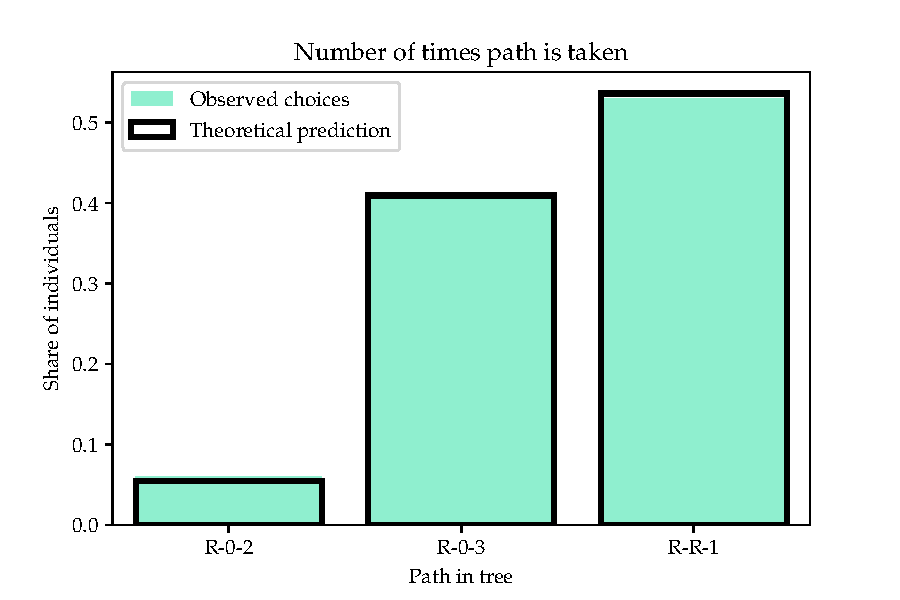
\includegraphics[width=\linewidth]{03_figures/choice_fractions_NL.pdf}
  \end{subfigure}
  \begin{subfigure}{0.45\linewidth}
    \caption{CNL}
    \centering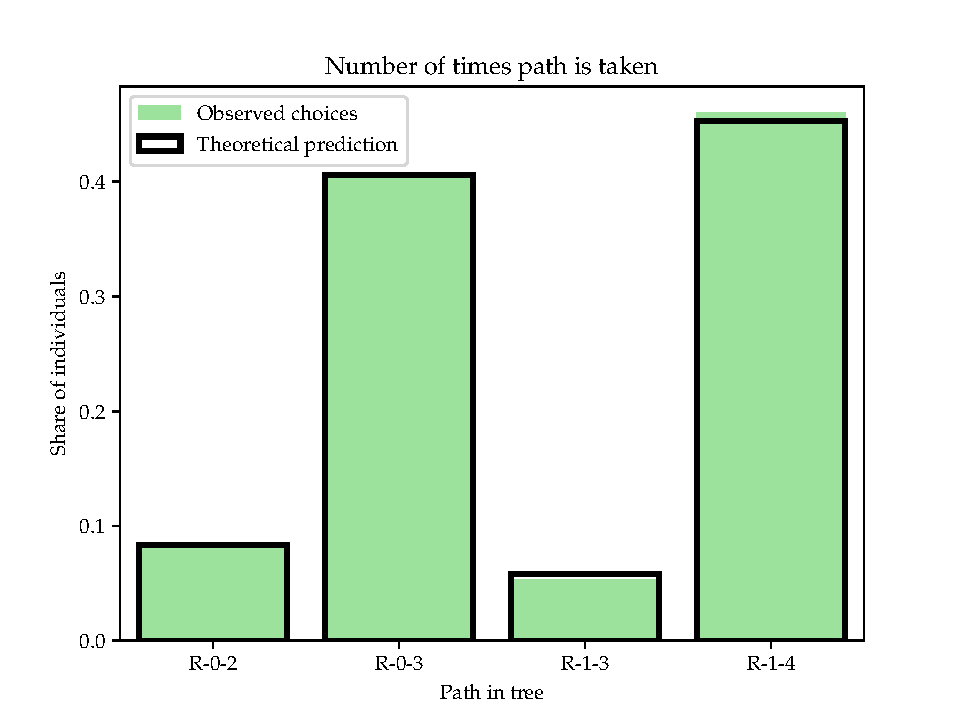
\includegraphics[width=\linewidth]{03_figures/choice_fractions.pdf}
  \end{subfigure}
  \caption[Actual and theoretical choice probabilities.]{Actual and theoretical choice probabilities. The x-axis is read as follows. From left to right is the path through the tree, with $R$ being the root, and apart from that the mapping is $(n_1, n_2, c_1,c_2,c_3) \rightarrow (0,1,2,3,4)$.}
  \label{fig: choiceprobs}
\end{center}
\end{figure}

By simulating and selecting data as described above we construct a dataset of 100 "individuals", and their hypothetical decision at every node of the CNL tree depicted in figure \ref{fig: simpletree}. The expected probability of a given path (i.e. $R\rightarrow n_1 \rightarrow c_2$) is then given by the product of nest-conditional probabilities at each step, and we can quite easily calculate these. Since we simulate the entire structure and not just the lowest nodes, we can trace out otherwise un-separable paths in the tree. Figure \ref{fig: choiceprobs} shows the observed share of choosers following a given path in the CNL tree and compares it to the theoretical number. First of all, the apparent dissymmetry of the CNL path shares compared to the ones in the NL model is useful in understanding the flexibility of the CNL model. Secondly this figure serves as a way of validating that our code functions as anticipated.


\subsection{Data validation}
We use a number of tests to ensure the DGP is correctly implemented. These all rely on the various probabilities debated in the section on estimation. Specifically we know that the following identities must hold true
\begin{equation}
  \begin{split}
  &\sum_{i\in \mathcal{C}} \textrm{Pr}(i|\mathcal{C}) = 1 \\
  &\sum_{m\in \mathcal{M}} \textrm{Pr}(m|\mathcal{C}) = 1
  \end{split}
\end{equation}
And finally we also know $\forall m : \ \sum_{i \in m} \textrm{Pr}(\mathcal{J} = i | m) = 1$. That is 1) the summed probability of making choice $i$ over the entire choice set must be 1, 2) the summed probability of entering nest $m$ summed over all nests must be 1 and 3) Within all nests, the summed probability of choosing $i\in m$ must be 1 when conditioning on being in the specific nest.
\\ \\
Knowing that our code passes all of these criteria we are confident that we simulate data from the correct DGP.

\subsection{Real data (the DREAM dataset)} \label{subsec: dreamdata}
In order to model probabilities regarding the course of those that are out of the labour market on sick leave, we use weekly data from the semi-governmental institution \textit{The Danish Institute for Economic Modelling and Forecasting}, the DREAM Group, based on their agreement with LO, The Danish Confederation of Trade Unions. More specifically the december 2017-version of the microeconometric database covering week-by-week socioeconomic status of all 5,6 million Danish citizens subdivided into 36 labour market categories. The registry lays the foundation for their socioeconomic projection model \citep{dream_danish_2018}. Table \ref{tab:sumstats} show summary statistics for the sample.

For simplicity we model the one-year course for the group of 84.123 persons on sick leave that received unemployment benefits ("sygedagpenge") in week 48 of 2016 (last week of november). Thus, the selection besides from being those hit by prolonged illness is limitied to those that have been a member of an unemployment insurance fund and have been in work recently in order to fulfill the conditions for receiving unemployment benefits.

\begin{table}
  \centering
\begin{tabular}{lrrr}
\toprule
{} &         $c_1$ &         $c_2$ &         $c_3$ \\
\midrule
All       &  0.12 &  0.35 &  0.53 \\
Male      &  0.11 &  0.34 &  0.55 \\
AC        &  0.11 &  0.27 &  0.62 \\
Age 15-30 &  0.14 &  0.26 &  0.60 \\
Age 30-40 &  0.13 &  0.32 &  0.55 \\
Age 40-50 &  0.11 &  0.35 &  0.54 \\
Age 50-60 &  0.11 &  0.40 &  0.49 \\
\bottomrule
\end{tabular}
\caption{Summary statistics: distribution of choices for subgroups in data.}
\label{tab:sumstats}
\end{table}

Our dataset is then reduced to 73.864 individuals by dropping the 10.259 above 60 years olds ultimo november 2017 in order to avoid interference with ordinary retirement schemes. Furthermore 6.348 are dropped who in week 48 of 2017 (last week of november) where on either paternity leave, no longer living in Denmark, dead, or neither employed nor receiving unemployment benefits (i.e. no information on one's livelihood).
\\ \\
We end up with 67.516 observations for which the following regressors are included:
  \begin{equation} \label{eq: DREAM_regressors}
    x = \left[\textrm{male, ac, age, age}^2\right]
  \end{equation}
Where \textit{ac} is a dummy for the 7 pct. of individuals in the dataset who are members of one of the four unemployment insurance funds for college graduates (\textit{AJKS}, \textit{AKA}, \textit{CA} or \textit{MA}).
\\ \\
The choices are defined based on their socioeconomic status in week 48 in 2017 (one year after having been on sick leave).
  \begin{itemize}
    \item[$c_1$] (\textit{"Ordinary unemployment"}): Receiving unemployment benefits while actively seeking jobs.
    \item[$c_2$] (\textit{"Sick"}): On sick leave ("sygedagpenge"), early retirement due to sickness ("førtidspension"), subsidized work on reduced hours due to sickness ("fleksjob"), or being in one of several courses for partially sick where one's amount of work-ability is examined.
    \item[$c_3$] Ordinary employment or under education.
  \end{itemize}
As the linear RUM setup (equation \ref{eq: utility_general}) is based on utility maximizing agents, our estimation model is to assume that the choice between $c_1$ and $c_3$ depends on the opportunity cost of being out of labour, i.e. as men and college graduates in general earn above the median wage we use these dummies as proxies for having a higher utility from choosing $c_3$ relative to $c_1$, besides from the other characteristics associated with ticking theese boxes which also for the most part drag in the direction of $c_3$. As a higher age is also correlated with a higher wage we similarly can expect older people to have a higher probability of choosing $c_3$ while a squared term for age allows for nonlinearity such that there could exist a maximum point for age from which on the probability of choosing $c_3$ over $c_1$ could be decreasing instead. Leaving the world of utility maximizing individuals for a second, the employer's side of an imperfect labour market might also have preferences regarding an employer's ideal age that can be described by a similar 2nd order polynomial which would further increase the effect. Given expectations about different probabilities for $c_1$ and $c_3$ based on regressors we assume that the error terms tend towards being uncorrelated and that there should not exist cross-nesting between this pair of alternatives.

$c_2$ on the other hand is difficult to fit into the RUM-setup. Thus we assume that being too sick to be available for the ordinary labour market is mainly correlated with a higher age while correlation with the other regressors is less significant. Assuming a near random draw of those hit by a more permanent sickness, we expect the hidden attributes in the error term to be both correlated with both those who choose $c_1$ and $c_3$ and thus we allow for cross-nesting with both nest $n_1$ and $n_2$, see the CNL-structure in \ref{fig: simpletree} above.


\section{Application to simulated data}
\label{sec: Code}

Simple econometric models can be estimated in a reasonable amount of time on even very modest computers, but as complexity grows estimation becomes increasingly challenging. While there are optimization routines that can optimize the CNL likelihood in reasonable time, implementing these routines is beyond the scope of this paper. For properly efficient estimation the only real option is one of the two specialized tools \textit{Biogeme} and \textit{Larch}. In all of the following we restrict one parameter in each nest to it's true value before estimation, we also assume $\alpha$ and $\mu_m$'s to be fixed at their true values.
\\ \\
We implement reasonably fast versions of the probability equations in \ref{eq: likelihoodderiv}, as well as implementations of $P(m|C)$ and $P(i|m)$ using Numpy in python 3.6. Evaluating the likelihood function in a single point takes approximately 6-7 seconds when using 1.000 observations. As the number of observations increase this process slows further as evident in table \ref{tab: loglikspeed}. This is a major obstacle for estimation, as the large number of parameters, and the complicated effects from parameters on the likelihood, means many observations are generally required to get accurate results.  Optimizing the $J\times K$ parameters jointly fails to converge when using the standard SciPy minimization routine. We do show some results from joint estimation, but one should note that these are from non-converging optimizers.

\begin{center}
\begin{threeparttable}
  \centering
  \caption{Speed comparison five evaluations of $\log\mathcal{L}_K$ at different data sizes}
  \label{tab: loglikspeed}
  \begin{tabular}{lrrrrr}
\toprule
{} &  Obs=10 &  Obs=50 &  Obs=100 &  Obs=1000 &  Obs=5000 \\
\midrule
0 &     1.0 &    5.02 &    10.23 &    124.15 &   1497.02 \\
\bottomrule
\end{tabular}

  \begin{tablenotes}\footnotesize
     \item Numbers are summed time over five iterations of $\log\mathcal{L}_K(\beta, \Theta; x)$ over the dataset with $\alpha$ set to the CNL structure and $\beta$ as described. Units is the running time relative the running time of the $K=10$ dataset. The running time when $Obs=10$ is approximately $0.35$ seconds.
  \end{tablenotes}
\end{threeparttable}
\end{center}

In the following we attempt to estimate model parameters in the CNL model through two very weak, but conceptually simple mechanisms. Especially the first attempt is very unlikely to produce unbiased estimates, let alone estimates that converge. The purpose of showing these attempts should thus not be seen as trying to argue that these methods are in general useable, but to explore the options for estimation in models which are so complex it requires specialist knowledge to code up estimators.

\subsection{Iterative estimation} \label{sec: iteropt}
The perhaps simplest way of estimating the model parameters is the following scheme. We assume that both $\alpha$'s, $\mu$ and $\mu_m$ are known and fixed to their true value. Recall that there is a $\beta$ for each $x$ for every choice (with some set to $0$), so we can arrange $\beta$ as a matrix of size $J\times K$.

\renewcommand{\kbldelim}{(}% Left delimiter
\renewcommand{\kbrdelim}{)}% Right delimiter
\begin{equation} \label{eq:matrices}
  \beta =
  \kbordermatrix{
    & \bm{\beta_0} & \bm{\beta_1} \\
    n_1 & \beta_{00} & \beta_{01} \\
    n_2 & \beta_{10} & \beta_{11} \\
    c_1 & \beta_{20} & \beta_{21} \\
    c_2 & \beta_{30} & \beta_{31} \\
    c_3 & \beta_{40} & \beta_{41} \\
  }
\hookrightarrow
  \kbordermatrix{
    & \bm{\beta_0} & \bm{\beta_1} \\
    n_1 & \beta_{00}^* & \beta_{01}^* \\
    n_2 & \beta_{10}^* & \beta_{11} \\
    c_1 & \beta_{20}^* & \beta_{21} \\
    c_2 & \beta_{30}^* & \beta_{31}^* \\
    c_3 & \beta_{40}^* & \beta_{41} \\
  }
\end{equation}

Our iterative optimization scheme then initialized $\beta^{\textrm{init}} = \bm{\beta^*}$, sets $\beta^{\textrm{init}}_{i0}$ to one as initial value, except for the parameters of choices $c_0$ (which is structural) and $c_3$ which are set to their true values. This is in accordance with the identification stategies outlines in section \ref{sec: Estimation} and illustrated by the right hook arrow in equation \eqref{eq:matrices}. Even though this significantly reduces the number of parameters the Scipy minimizer is still not able to converge when maximizing the likelihood w.r.t the full set of free parameters. We then iteratively optimize each element of $\beta$ assuming all other elements fixed. After each iteration $\beta$ is updated to include the found optimal value. This process is then carried out in a loop until the change in the entire $\beta$ matrix from $t$ to $t+1$ is sufficiently small. In pseudocode a single iteration over the matrix would look like

\begin{algorithm}[H]
  \label{algo:iteroptimizer}
  \SetKwInput{Precondition}{Precondition~}
  \SetKwInput{Input}{Input~}
  \SetKwInput{Data}{Data~}
  \SetKw{Continue}{continue}
  \SetKw{In}{in}

  \caption{Iterative Optimizer}

  \footnotesize
  \DontPrintSemicolon
  \Input{\texttt{$\beta$}: A matrix of parameter vectors}
  \Input{\texttt{$C$}: A vector of choice indices}
  \ForEach{parameter $\beta_i$ \In $\beta$}{
    \ForEach{ choice $c_i$ \In $C$}{
      $\beta_{[b][c]}^*$ = \texttt{OptimizeScalar}($\log\mathcal{L}^{i|\mathcal{C}}_K(\beta, x, \Theta)$) w.r.t $\beta_{[b][c]}$ \\
      $\beta_{[b][c]} \leftarrow \beta_{[b][c]}^*$
    }
  }
\end{algorithm}

As mentioned this process is carried out repeatedly over the continuously updating matrix. Of course this estimation approach is not ideal, but computationally it is feasible to implement within the scope of this paper. For each iteration over the matrix we update the parameter space to be searched, to a slightly narrower segment recentered around the current value of $\beta_{[b][c]}$.

\begin{figure}[h]
  \centering
  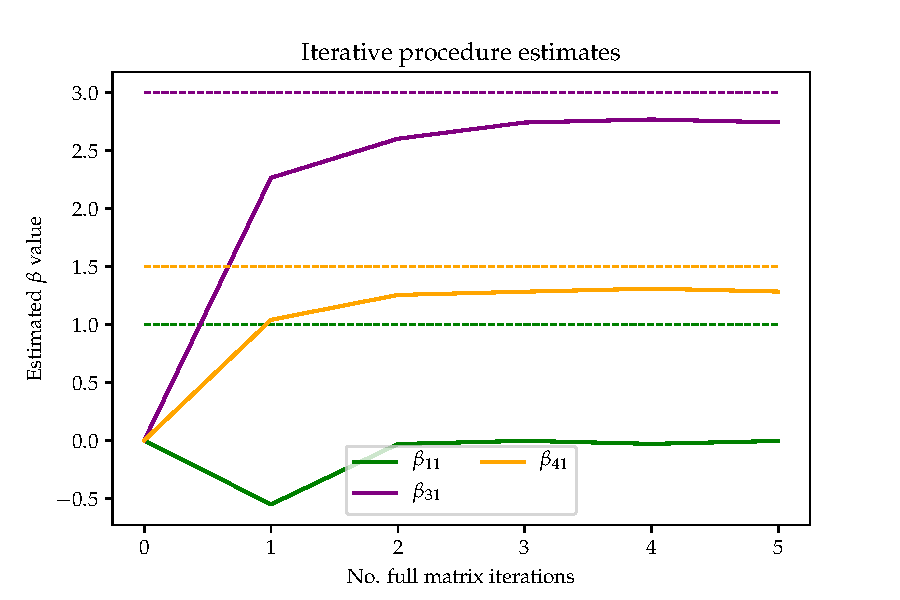
\includegraphics[width=0.8\linewidth]{03_figures/iterEstimate.pdf}
  \caption[Parameter development using iteration.]{Parameter development using iteration. Dashed lines are true parameter values. Each step on the first axis corresponds to a full loop of algorithm \ref{algo:iteroptimizer} over the $\beta$-matrix.}
  \label{fig: iterbetas}
\end{figure}

An intuitive argument for why this method will at least in some cases converge is that if each single-dimensional optimization moves the estimated $\beta$ closer to it's true value, it improves the conditions for estimating the other $\beta$'s in the following iteration bringing them closer to their optimum as well. Thus in the end parameters should converge on their true values. For this to be the case it is essential that the sub-routines consequently move estimates closer to their true values, which will only be the case if the likelihood function is dimensionwise concave, as it is otherwise possible for estimates to move away from their true values in the subroutines. More formally if $\mathcal{L} : \mathbb{R}^n \rightarrow \mathbb{R}$ is a likelihood function dependent on $n$ parameters $\beta$, then if every cross-section of $\ell = \mathcal{L}(\beta_i | \beta_{-i}, \Theta, x)$, $\ell : \mathbb{R} \rightarrow \mathbb{R}$  has a single optimum (implying the function is strictly concave for some sign) and the full function $\mathcal{L}$ has a single optimum as well, then the optima found in $\ell$ after each iteration will converge to the global optimum. This is because 1) the optima in $\ell$ cannot be lower than the global optimum in $\mathcal{L}$, 2) there must be at least one dimension in which a non-global optimum is deviated from (otherwise the function would have local optima) and 3) this deviation will always happen in the direction of the global optimum, as otherwise it would constitute a local optimum. On the other hand in the absence of these rather strict requirements for $\mathcal{L}$ it is intuitive that this kind of optimization will fail.

From figure \ref{fig: iterbetas} it is clear that this simple method suffers from a variety of biases and divergence issues. However this was to be expected. The quick stabilization of estimates might be a sign that the algorithm very quickly approaches a local minimum, which works as an attractor, preventing convergence to the true value. A more formal proof that this is not purely coincidental is needed, but our preliminary testing does provide some circumstantial evidence of (biased) convergence.


\subsection{Joint and nest based optimization}
As an alternative to the naive method implemented above we also attempt a nest based solution, in which we formulate a likelihood based on $\textrm{Pr}(i|m)$ instead of using $\textrm{Pr}(i|C)$ as above. This is in essence the same as considering each choice as it's own $\alpha$-augmented multinomial trial, and therefore requires information on the structural choices. Like with the iterative optimizer this approach is not ideal as coefficients are not restricted across nests, meaning we can get different $\beta$ estimates for cross nested choices, depending on the step of the optimization problem. In exchange the likelihood is significantly simpler, meaning estimation can happen in feasible time.

\begin{figure}[h]
  \centering
  \includegraphics[width=0.8\linewidth]{03_figures/jointEstimation.pdf}
  \caption[Estimate deviations $\beta^* - \hat{\beta}$]{Estimate deviations $\beta^* - \hat{\beta}$ for the nest-based optimization, as well as a joint estimation using the full likelihood.}
  \label{fig: nestandjoint}
\end{figure}

Figure \ref{fig: nestandjoint} show parameters in deviations from their true values when applying the nest-based optimization, as well as (non-convergent) optimization results from attempting to optimize the full likelihood. In both cases we implement the same parameter restrictions as in section \ref{sec: iteropt} for comparison. We take the results as yet another indication that these iterative optimizers are not ideal, but also note that even though the build in Scipy optimizer fails to converge, the results it find are not far from the true values of $\beta$. Actually the Scipy optimizer seems to be about as accurate as our iterative procedure, and the nest based method good only for some parameters. Thus slight improvements in the code might provide good estimates, granted the right parameter restrictions are implemented for identification.

\subsection{Marginal effects in simulated data}
Marginal effects are usually studied in relation to the regressors - that is the question is, if we alter a specific independent variable slightly, what will the resulting change in choice probabilities be. Small changes in specific $\beta$'s are however perhaps even more interesting in a simulation setting, as it is the parameters that vary across choices in the multinomial CNL model. Panel (a) in \ref{fig: marginalities} show for each of 1000 simulated individuals their probability of choosing the cross nested alternative $c_3$ as the $\beta$'s related to the structural nodes $n_1$ and $n_2$ are varied (left and right column respectively). These naturally vary between individuals as the $x$-value is specific to them, meaning a change in $\beta$ affects them differently. The apparent diversity in these curves for different values of $\beta$ is due to the complex changes in $P(i|\mathcal{C})$ when $x$ is either positive or negative, as well as the changes occurring when $|x|\lessgtr 1$.

\begin{figure}[h]
  \begin{center}
  \begin{subfigure}{0.45\linewidth}
    \centering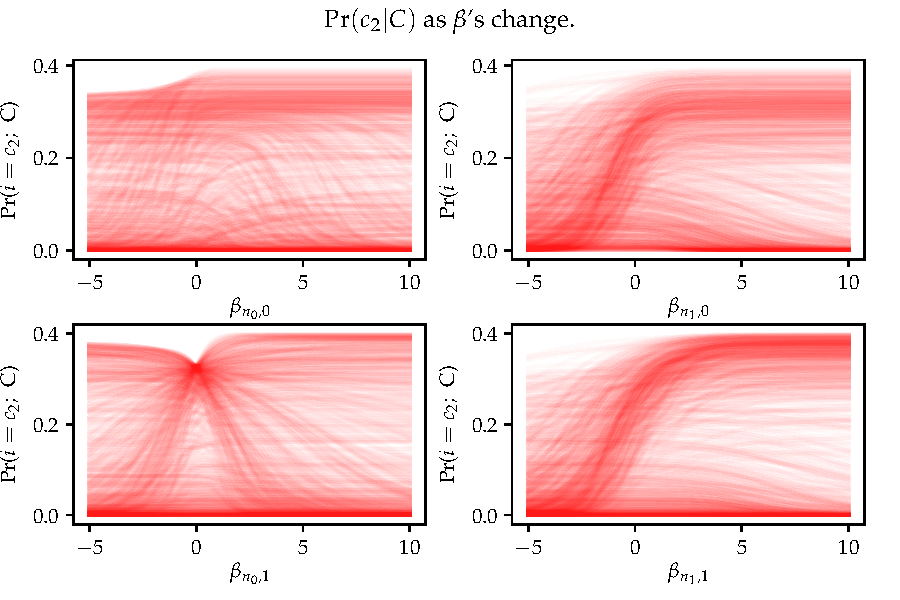
\includegraphics[width=\linewidth]{03_figures/beta_effect.pdf}
    \caption{Individual probabilities as function of $\beta$'s}
  \end{subfigure}
  \begin{subfigure}{0.45\linewidth}
    \centering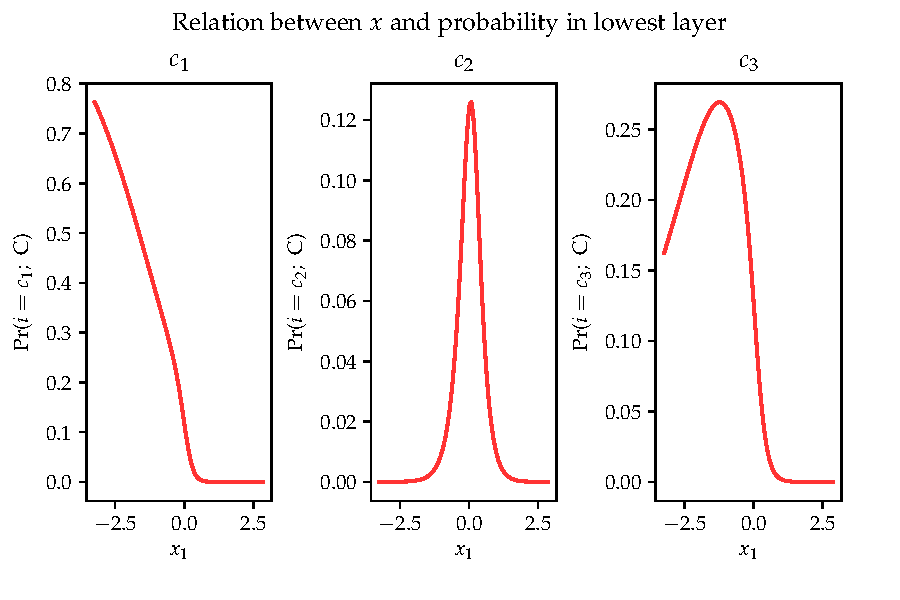
\includegraphics[width=\linewidth]{03_figures/marginaleffects.pdf}
    \caption{Population effects of altering $x_1$ by a constant}
  \end{subfigure}
  \caption{Variations in $P(i|\mathcal{C})$ when altering $\beta$'s and $x$'s}
  \label{fig: marginalities}
\end{center}
\end{figure}

The right panel on the other hand shows choice probabilities as a function of data, specifically $x_1$. These probabilities are naturally identical across the population for a given $x$. The normally considered marginal effects, $\partial p_i / \partial x_i$ is the derivative of these curves. Figure \ref{afig: nl_marginalities} show a plot similar to the one in figure \ref{fig: marginalities} panel (b), but calculated in the nested logit depicted in figure \ref{fig: simpletree}.
\\ \\
Naturally there are many more cross-effects than those shown here. These can easily be constructed by refering to the supplied code.\footnote{The code will be made available on \url{https://github.com/Kristianuruplarsen} after the paper has been graded.} Figure \ref{afig: marginalities} show similar figures but for $\textrm{Pr}(i|m)$, this shows clearly how when conditioning on the specific nest, the probability of making any of the choices are essentially inversely related as in the regular logit.


\section{Application to real data}
\subsection{Estimation on DREAM data}
In the following we estimate MNL, NL and CNL models on the DREAM data described in section \ref{subsec: dreamdata}.
For the estimation we use Larch, which uses two optimization routines SLSQP and BHHH to estimate utility parameters as well as a number of nesting related parameters. There is no real consensus about whether structural nodes should be assigned linear utility or simply represent components of the error terms. Larch does not directly model structural utility, but instead lets the utility of choosing a specific nest be\footnote{\url{http://larch.readthedocs.io/en/latest/math/aggregate-choice.html}}
\begin{equation}
  V_{m} = \mu_{m} \left( \sum_{j} \alpha_{im} \exp \left( \frac{V_i}{\mu_m}
  \right) \right)
\end{equation}
Where $\mu_m$ is then estimated. That is the independent utility from structural nodes, is simply the weighted sum of utilities available from children of the given nest. Furthermore to estimate the cross nested $\alpha$ parameter, Larch uses a logit-like link function\footnote{\url{http://larch.readthedocs.io/en/latest/example/111_cnl.html}} like
\begin{equation}
  \alpha_{im} = \frac{\exp(\phi_{i} Z )}{\sum_j \exp(\phi_j Z)}
\end{equation}
to avoid dealing with optimization constraints, while still ensuring $\alpha_{im} \in [0,1]$. naturally this defaults to $0.5$ when not specified, equivalent to setting $Z = 0$. In \ref{tab: results} we report a CNL model with the default setting of $Z = 0$ to simplify the results as much as possible. Results are however robust to the inclusion of this specification.
\\ \\
For identification we attempt a strategy similar to the one used in the iterative optimization routine, setting all parameters related to $c_1$ to $0$ (we used the true values when simulating, but this is only to help our less sophisticated optimizers), and one parameter in each $c_i$ = $0$. This effectively normalize the utility of each choice, with a baseline of one, as well as normalizing the utility of each nest, also with a baseline of one.
\\ \\
Table \ref{tab: results} show estimated parameters in MNL, NL and CNL models on the DREAM data described in section \ref{subsec: dreamdata}. First note that for the NL model $\mu_m$ is estimated to 1, as would be expected since there is only one nest. In the CNL model we do not estimate any $\alpha$'s but instead estimate the logsum parameters to be $0.6$ and $0.96$ respectively. In all three models, the square of age is very close to $0$, while age in itself is only really important in the NL model. In general it is difficult to compare these estimates directly.
Like in the MNL all of these estimates are best interpreted by calculating marginal effects at the mean, but for both the NL and CNL models, these are complicated functions dependent on $G$'s derivatives as we have shown in section \ref{sec:marginalderivation}.

\begin{table}
  \centering
  \footnotesize
\begin{tabular}{c|ll|ll|ll}
  \toprule
           & \multicolumn{2}{c}{CNL}    & \multicolumn{2}{c}{NL}      & \multicolumn{2}{c}{MNL}                \\ \hline
     parameter &      $\beta$ &        $t$-value &       $\beta$ &         $t$-value &         $\beta$ &           $t$-value \\
\midrule
ASC$_2$      &    -0.412 &  -2.344 &   13.053 &  33.174 & -0.578 & -2.661 \\
ASC$_3$      &     1.012 &   5.648 &  -88.537 & -61.640 &  1.053 &  5.249 \\
age$_2$      &     0.048 &   5.660 &   -0.581 & -32.905 &  0.058 &  5.419 \\
age$_3$      &     0.014 &   1.561 &    5.833 &  66.572 &  0.018 &  1.859 \\
agesq$_2$    &    -0.000 &  -3.712 &    0.007 &  36.513 & -0.000 & -3.420 \\
agesq$_3$     &    -0.000 &  -1.754 &   -0.091 & -69.004 & -0.000 & -1.729 \\
AC$_2$       &    -0.163 &  -3.739 &   -3.318 & -55.419 & -0.209 & -3.838 \\
AC$_3$       &     0.262 &   5.945 &   11.220 &  52.640 &  0.238 &  4.782 \\
Male$_2$     &     0.016 &   0.769 &   -0.331 & -10.520 &  0.020 &  0.761 \\
Male$_3$     &     0.108 &   4.826 &    6.618 &  61.748 &  0.113 &  4.419 \\
$\mu_1$       &     0.755 &  32.108 &    1.000 &     - &    - &    - \\
$\mu_2$       &     0.962 &  -1.738 &      - &     - &    - &    - \\ \hline
Iterations & \multicolumn{2}{c}{64}      & \multicolumn{2}{c}{61}      & \multicolumn{2}{c}{4}                \\
AIC & \multicolumn{2}{c}{-2.137}      & \multicolumn{2}{c}{-4.882}      & \multicolumn{2}{c}{1.866}                \\
Optimizer  & \multicolumn{2}{c}{SLSQP}   & \multicolumn{2}{c}{SLSQP, BHHH}   & \multicolumn{2}{c}{BHHH} \\
\bottomrule
\end{tabular}
\caption[Optimization results]{Optimization results, DREAM data. Subscripts denote the choice  $c_i : i \in2,3$ for which the parameter is calculated, except for $\mu$ where they identify nests.}
\label{tab: results}
\end{table}

Some authors \citep{hausman_specification_1984, koppelman_self_2006}) propose using likelihood ratio (LR), Wald, or Lagrange multiplier tests for model selection by comparing an estimated NL model to the MNL model that can be specified as a special case of the more general NL model. On the surface this might seem reasonable to apply to CNL models as well. We have shown the GEV framework nests both MNL, NL and CNL models, and that one way of representing this is trough the $\alpha$ matrix. However, using LR tests does not account for the fact that $\alpha$'s are co-linearly dependent, nor for the fact that the choice set $\mathcal{C}$ is altered when moving from e.g. a NL model to a MNL model. This alteration of the choice set, means the models are not algebraically nested as is required in the LR test. Instead MNL is only nested when we allow for set operations.
\\ \\
The justification for using LR tests is weak as it does not take these considerations into account. Instead of LR values, we therefore calculate the Akaike Information Criterion\footnote{$AIC = 2k - 2 \ln(\hat{\mathcal{L}})$ with $k$ being the number of parameters estimated and $\hat{\mathcal{L}}$ the maximum of the likelihood.}, which does not require models to be nested.
\\ \\
We find that while AIC's are close, the lowest AIC is achieved by the NL model indicating that nesting $c_1$ ordinary unemployment benefits and $c_2$ being on sick leave, or various other benefits is the best of the three models. This is intuitive as the third category $c_3$, ordinary employment is a choice probably made by a different type of individuals than those who end up in either $c_1$ or $c_2$. One interpretation of these results is that there is selection between $c_1,c_2$ and $c_3$. In other word there seems to be some selection into the nest of unemployment among those who were on sick leave one year prior. Why this might be the case is left for future research, as this question is probably not suitable for answering within the GEV framework.
The model does not give an answer as to whether this selection is driven by the individuals, as an alternative explanation could be that it is a sampling effect, where those in the nest share traits such as high age, making it difficult for them to get into employment and overcome severe sickness respectively. A bias might also arise from the effect that it is not solely up to the individual to decide on which benefits to receive, producing a high degree of substitution within the social benefit nest if some individuals are misplaced in the benefits system.


\section{Perspectives}


% \subsection{Estimation results}
% In order to increase the predictability it would be necessary to include more background variables through merging the DREAM dataset with registries such as TIMES from Statistics Denmark containing background variables like prior income. A first issue would be that it is practically impossible to write Python code on the servers of Statistics Denmark, another issue is the trade-off between estimation time and the level of detail in terms of the number of regressors.

\subsection{Results}
We manage with some success to estimate CNL parameters even with low-performance estimation techniques, however the convergence of these methods is highly dependent on their initiation state, and the data at hand. For future work estimators must be implemented in a faster language, which is more suitable for heavy computation. Given that one does implement CNL in a better framework however, there are plenty opportunities for research, either into the interpretation of model output, or in the behavior in the model under various types of biases and data.
\\ \\
When applying the model to real data, we're faced with the issue of interpretability, and resort to the AIC for our conclusions. Using the Akaike Information Criterion we find some evidence of nesting in the choices of individuals who have been on sick leave, and in particular find that there is an "unemployment nest" in the choice structure. How robust these results are is difficult to say, given the complexity of the model, and future work could investigate the validity of conclusion drawn on the basis of NL and CNL models.

\subsection{Usability and interpretability of CNL}
While CNL will surely have applications in some areas of economics and other sciences, it is unlikely to gain widespread use, as estimation is restricted to a few software packages, which are relatively poorly documented and extremely difficult to modify. Implementing a maximum likelihood estimator of the likelihood is feasible for experts, but doing so will sacrifice transparency of methodology. A recent paper by \citet{mai_dynamic_2017} suggests borrowing methodology from the field of dynamic programming for estimation, and development of pre-coded solutions for these methods can possibly increase accessibility to the GEV models.
\\ \\
Advances in computation will however not make interpretation of results easier, and from the figures \ref{fig: marginalities} and from the marginal effects in equation \eqref{eq: marginaleffects} it is clear that marginal effects are not guaranteed to be monotone in neither parameters or regressors, making truthful reporting very difficult.


\section{Conclusion}

In this paper we have presented the Cross-nested Logit (CNL), through a thorough review of less complex models in the GEV family, and a GEV-oriented description of the features and limitations of the cross nested logit model. In this regard we contribute primarily known material. We also show a number of derivations, e.g. the marginal effects in equation \eqref{eq: marginaleffects} and the properties for substitution patterns in section \ref{sec: iiaproof}, which are perhaps to concrete to have been of interest in previous work, but has a very direct link to the ordinary logit models.
\\ \\
We simulate data from both nested and cross-nested structures, and implement two relatively naive estimation techniques as computational difficulties hinder a full likelihood estimation.
\\ \\
The paper also contains discussions on the usability of the cross nested models, and implements a simple model on real data from the Danish DREAM database. In this regard we find that while there is with no doubt lessons to be learnt from complex structural modelling. However the estimates suffer in interpretability and transparency, why we foresee some waiting before the CNL gains widespread use. We find evidence that nesting is a better model specification for the data (see section \ref{subsec: dreamdata}), than MNL suggesting that those on sick leave at time $n$ will one year later act in accordance with a nested structure with a node for employment, and a nest covering various states of unemployment.


\clearpage
\printbibliography
\clearpage


\appendix
\renewcommand\thefigure{\thesection.\arabic{figure}}
\setcounter{figure}{0}

\setcounter{page}{1}
\pagenumbering{roman}


%%% File encoding is ISO-8859-1 (also known as Latin-1)
%%% You can use special characters just like �,� and �

\section{Figures}

\begin{figure}[h]
  \begin{center}
    \centering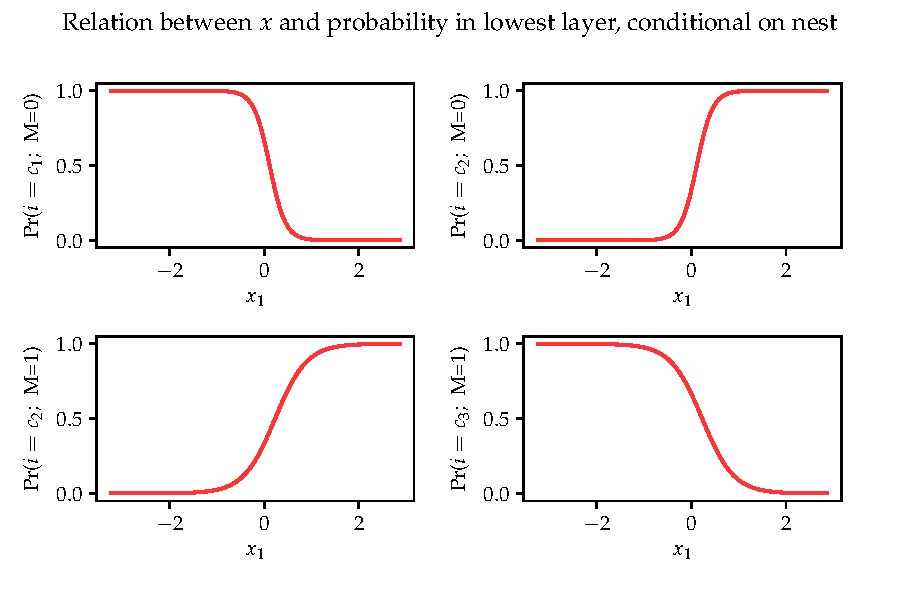
\includegraphics[width=\linewidth]{03_figures/marginaleffects_on_M.pdf}
    \caption{Individual probabilities as function of $\beta$'s, conditional on $m$}
  \label{afig: marginalities}
\end{center}
\end{figure}



\begin{figure}[h]
  \begin{center}
    \centering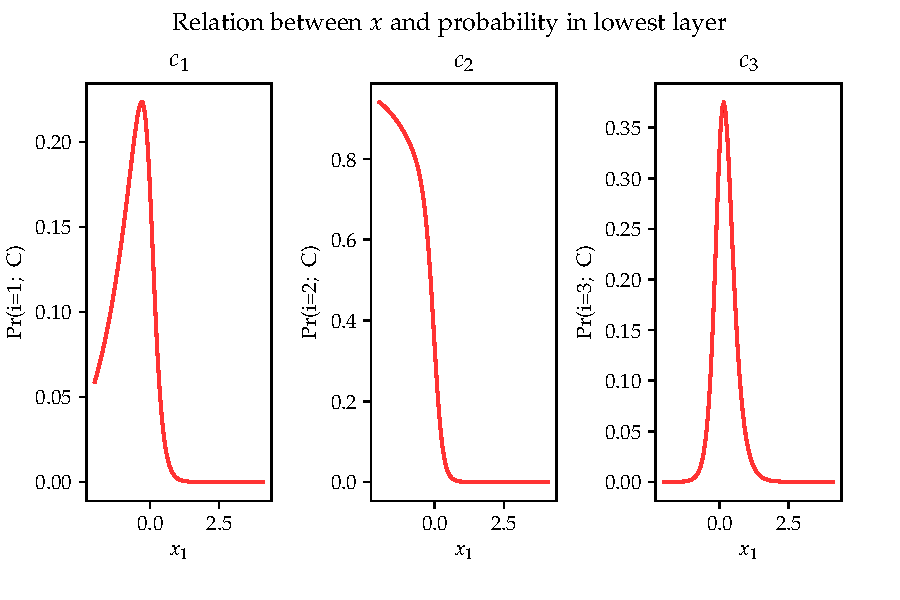
\includegraphics[width=\linewidth]{03_figures/marginaleffects_NL.pdf}
    \caption{Relation between $x_1$ and choice probabilities in the Nested Logit model}
  \label{afig: nl_marginalities}
\end{center}
\end{figure}

\clearpage
%%% File encoding is ISO-8859-1 (also known as Latin-1)
%%% You can use special characters just like �,� and �

\FloatBarrier
% \section{Examples of substitution patterns}
% \label{sec: examples}
% In the following we clarify the thorough implications of the \textit{Independence of Irrelevant Alternatives} (IIA) by analyzing how different choice structures lead to fundamentally different predictions for the reaction to new choices being added in terms of potential changes in the ratio of probabilities between the existing alternatives.

\section{Commuting-example for the MNL model}
\label{sec: MNL_example}
Inspired by \citet{koppelman_self_2006} the starting point is the commuters choice between $car$ and $bus$ as the two possible means of transport in a choice set $\mathcal{C}^0$ for everyday commuting to work. Say that the commuter given her characteristics would choose to drive alone in a car with probability $\frac{2}{3}$ and to take the bus with probability $\frac{1}{3}$, thus, the ratio of probabilities is
  \begin{equation} \label{eq: bus_car}
    \frac{\textrm{Pr}(\mathcal{J}=\textrm{car}|\mathcal{C}^0)}
    {\textrm{Pr}(\mathcal{J}=\textrm{bus}|\mathcal{C}^0)}=
    \frac{2/3}{1/3}=2
  \end{equation}
Now let us say a railway is being build and a local $train$ line is introduced with several stations not far from the bus line used by the commuter. Furthermore the same ticket system applies for both of the public transport alternatives.


  \begin{figure}[!h]
    \begin{center}
    \def\svgwidth{0.70\columnwidth}
    \import{03_figures/}{MNL.pdf_tex}
    \caption{Examples of Multinomial Logit models for two choice sets. \\
    For our analogy $c_1$ is bus, $c_2$ is train, and $c_3$ is car.}
    \label{fig: MNL}
    \end{center}
  \end{figure}


Looking at this new choice set $\mathcal{C}$ in figure \ref{fig: MNL} let us first assume for simplicity that the commuter with a RUM-type utility function (\ref{eq: utility_general}) would choose $train$ and $bus$ with equal probability as the two alternatives share somewhat similar characteristics (note though, that the probability of taking the train could be set to any number $\in]0,1[$ for this example to carry through).
  \begin{equation} \label{eq: train_bus}
    \textrm{Pr}(\mathcal{J}=\textrm{train}|\mathcal{C})
    =\textrm{Pr}(\mathcal{J}=\textrm{bus}|\mathcal{C})
  \end{equation}
In line with the IIA assumption the ratio of probabilities for
(\ref{eq: bus_car}) is kept constant, such that $\frac{2}{3}$ of the new train passengers took the car before and $\frac{1}{3}$ of the train passengers took the bus before as this was the distributions before the introduction of the train and IIA assumes equal competition. Take into account the probability of taking the $train$ (\ref{eq: train_bus}) and that the probabilities of the choices have to sum to one. The solution under these three conditions is that the probabilities of the extended choice set $\mathcal{C}$ should be
  \begin{equation} \label{eq: bus_car_train}
    \textrm{Pr}(\mathcal{J}=\textrm{car}|\mathcal{C})=\frac{1}{2},\ \ \
    \textrm{Pr}(\mathcal{J}=\textrm{bus}|\mathcal{C})=\frac{1}{4},\ \ \
    \textrm{Pr}(\mathcal{J}=\textrm{train}|\mathcal{C})=\frac{1}{4}
  \end{equation}
Thus, the MNL model predicts that the effect of adding another public transport option is that the probability of taking the $car$ drops from $\frac{2}{3}$ to $\frac{1}{2}$ while the joint probability of taking \textit{public transport} goes up from $\frac{1}{3}$ to $\frac{1}{2}$.

Implying that twice as many $train$ passengers took the $car$ before as opposed to the $bus$ makes it obvious that IIA is a wrong assumption in this case. That is, the MNL model overestimates the joint probability of taking \textit{public transport} due so keeping the prior ratio of probabilities between taking the car and taking the bus (\ref{eq: bus_car}) constant despite the introduction of a train-alternative.

Deviating from the IIA-axiom, a more realistic assumption (though extreme too) could be that $bus$ and $train$ are such similar alternatives that the introduction of a train line does not affect the probability of taking the $car$ but only takes over a share of the prior probability of taking the bus. The ratio of probabilities of the pair \textit{(car, bus)} (\ref{eq: bus_car}) would not be IIA in this case and would instead be expected to change.
% \\ \\
% , such that the joint probability of choosing a \textit{public transport alternative} is kept constant at $\frac{1}{3}$ and likewise the probability for taking the $car$ at $\frac{2}{3}$.
% In other words, the probability of taking the $car$ might be irrelevant of the addition of $train$ to the choice set, but the probability of taking the $bus$ is very unlikely to be irrelevant to adding a $train$-option. Thus, the ratio of probabilities of the pair \textit{(car, bus)} (\ref{eq: bus_car}) is not IIA in this case and would instead be expected to change.
% \\ \\
% While not very plausible, reality might show that by introducing a train line we would get a probability distribution not too far from (\ref{eq: bus_car_train}). Such a result could be explainable if $train$, while sharing some characteristics with the bus, also has some features different from the bus that makes it more attractive to the car-drivers (e.g. being able to work while commuting or both alternatives being more comfortable than the bus). Nonetheless, this would mean a double violation of the IIA-axiom that somehow about cancels each other out, as the individuals choosing train and car respectively would need to have some unobserved characteristics in common (e.g. having well-paid office-jobs or simply wanting to avoid less comfortable busses).
%
% Blue-bus/red-bus paradox
% One of the most classic examples of violation of the IIA assumption is classic "red bus/blue bus paradox" \cite{koppelman_self_2006}.
% The starting point is the commuters choice between car and a blue bus line as the means of transport for everyday commuting to work. Say that the commuter would take the car with probability $\frac{2}{3}$ and the blue bus with probability $\frac{1}{3}$, thus, the ratio of probabilities is
%   \begin{equation} \label{eq: blue_car}
%     \frac{\textrm{Pr}(\mathcal{J}=\textrm{car}|\mathcal{C})}
%     {\textrm{Pr}(\mathcal{J}=\textrm{blue bus}|\mathcal{C})}=
%     \frac{2/3}{1/3}=2
%   \end{equation}
% A competing bus company introduces a bus line on the same route with the only difference being that the bus is painted red instead of blue. Besides that the red bus line has the same characteristics as the blue bus line.
%
% Looking at this new choice set $\mathcal{C}'$ it is first of all clear that the utility optimizing commuter with a RUM-type utility function (\ref{eq: utility_general}) should choose blue bus and red bus with equal probability as they share the same characteristics
%   \begin{equation} \label{eq: blue_red}
%     \textrm{Pr}(\mathcal{J}=\textrm{blue bus}|\mathcal{C}')
%     =\textrm{Pr}(\mathcal{J}=\textrm{red bus}|\mathcal{C}')
%   \end{equation}
% In line with the IIA assumption the ratio of probabilities (\ref{eq: blue_car}) is kept constant. Take also into account the condition (\ref{eq: blue_red}) and that the probabilities of the choices have to sum to one. The solution under these three conditions is that the the probabilities of the extended choice set $\textrm{C}$ should be
%   \begin{equation} \label{eq: blue_red_car}
%     \textrm{Pr}(\mathcal{J}=\textrm{car}|\mathcal{C}')=\frac{1}{2},\
%     \textrm{Pr}(\mathcal{J}=\textrm{blue bus}|\mathcal{C}')=\frac{1}{4},\
%     \textrm{Pr}(\mathcal{J}=\textrm{red bus}|\mathcal{C}')=\frac{1}{4}
%   \end{equation}
% Thus, the MNL model predicts that the effect of adding another bus on the same route is that the probability of taking the car drops from $\frac{2}{3}$ to $\frac{1}{2}$ while the joint probability of taking any bus goes up from $\frac{1}{3}$ to $\frac{1}{2}$.
%
% It is obvious that IIA is a wrong assumption in this case. The ratio of probabilities between the probability of taking the car and taking the blue bus should not be kept constant when adding an alternative such as a red bus that is likely to be irrelevant to the probability of taking the car but certainly not irrelevant to the probability of taking the blue bus, thus the ratio of probabilities (\ref{eq: blue_car}) should not be expected to be constant.



% \subsection{Commuting-examples for the NL model}
% \label{sec: NL_example}
% Elaborating on the example for the MNL model in section (\ref{subsec: IIA}), still inspired by \citet{koppelman_self_2006}, we first consider the MNL-tree in figure \ref{fig: NL} where $c_1$ is taking the $bus$, $c_2$ is taking the $train$, and $c_3$ is to \textit{drive alone}. As pointed out in the MNL-example it is likely that $bus$ and $train$ have some attributes in common which could either be directly observed (by sharing an alternative-variant regressor like having the same cost in a joint ticket-system) or be unobserved while being represented in the error terms that would correlate (e.g. being more environmental friendly which could correlate with having a higher educational level, or not having a start-up cost as opposed to $car$ which could correlate with alternative-invariant regressors like having low income, being young, and/or female).
%
% To allow for correlation between $bus$ and $train$ we nest them together in a \textit{public transport} nest, $n_1$, as shown in the NL-tree in figure \ref{fig: NL}.
% \\
%   \begin{figure}[!h]
%     \begin{center}
%     \def\svgwidth{0.90\columnwidth}
%     \import{03_figures/}{NL.pdf_tex}
%     \end{center}
%     \caption{Examples of Nested Logit models for different structures and choice sets. \\
%     In our analogy $c_1$ is bus, $c_2$ is train, $c_3$ is drive alone (car), $c_4$ is shared-ride, $c_5$ is light-rail, and $n_1$ is a public transport nest.} \label{fig: NL}
%   \end{figure} \\
%   We analyze the choice set $\mathcal{C}$ and the addition of the option of choosing \textit{shared-ride}, $c_4$, giving us an extended choice set $\mathcal{C}'$. As a point of reference we make the strict assumption that \textit{shared-ride} is unnested and though does not have observed or unobserved attributes in common with any other alternative (as in the NL-tree for $\mathcal{C}'$ in figure \ref{fig: NL}). We will later loosen this restriction by introducing cross-nesting in section (\ref{sec: CNL_example}).
%
%   For now we consider the NL as a two-level process and take advantage of the fact that the \textit{bottom up method} gives consistent results \citep{train_discrete_2009}. Our lower model is the probability of choosing $bus$ or $train$ from the choice set $C_{n_1}$ given that we are in the \textit{public transport} nest $n_1$. Then for the upper model we do not observe $bus$ or $train$ directly but only observe \textit{public transport} as a possible choice, such that the choice set for the upper model (the root) $\mathcal{C}_R$ consists of \textit{public transport, drive alone}, thus $Pr(n_1|\mathcal{C}_R)=\sum\limits_{i\in\mathcal{C}_{n_1}}Pr(i|\mathcal{C})$.
%
%   Considering the two choice sets $\mathcal{C},\mathcal{C'}$ shown in figure \eqref{fig: NL} we can assume IIA for $(bus,train)$ as long as no sub-nest to $n_1$ exists. By the definition of $Pr(n_1|\mathcal{C}_R)$ we can assume IIA for \textit{(public transport, drive alone)} and \textit{(public transport, bus)} as the relative probability is unchanged for each of the pairs.
%
%   Now considering the upper model in $\mathcal{C},\mathcal{C'}$ we can assume IIA for \textit{(public transport, train)} as it is a simple MNL model. This would ensure that the relative probability would also be unchanged for \textit{(bus, drive alone)} and \textit{(bus, drive alone)} respectively which we prove as
%   \begin{equation} \label{eq: NL_IIA_proof}
%     \begin{split}
%      \frac{\textrm{Pr}(c_3|\mathcal{C})} {\textrm{Pr}(n_1|\mathcal{C}_R)}
%      =\frac{\textrm{Pr}(c_3|\mathcal{C'})} {\textrm{Pr}(n_1|\mathcal{C'}_R)}
%      \ \wedge\ & %&&
%      \frac{\textrm{Pr}(c_1|\mathcal{C})} {\textrm{Pr}(n_1|\mathcal{C}_R)}
%      = \frac{\textrm{Pr}(c_1|\mathcal{C'})} {\textrm{Pr}(n_1|\mathcal{C'}_R)}
%      \\ \Rightarrow
%      \frac{\frac{\textrm{Pr}(c_3|\mathcal{C})} {\textrm{Pr}(n_1|\mathcal{C}_R)}}
%      {\frac{\textrm{Pr}(c_1|\mathcal{C})} {\textrm{Pr}(n_1|\mathcal{C}_R)}}
%      =\frac{\frac{\textrm{Pr}(c_3|\mathcal{C'})} {\textrm{Pr}(n_1|\mathcal{C'}_R)}}
%      {\frac{\textrm{Pr}(c_1|\mathcal{C'})} {\textrm{Pr}(n_1|\mathcal{C'}_R)}}
%      \Rightarrow &\ %&&
%      \frac{\textrm{Pr}(c_3|\mathcal{C})} {\textrm{Pr}(c_1|\mathcal{C})}
%      \ =\ \frac{\textrm{Pr}(c_3|\mathcal{C'})} {\textrm{Pr}(c_1|\mathcal{C'})},\  \ \ \ \ \textrm{Q.E.D.}
%     \end{split}
%   \end{equation}
%   As long as the difference between $\mathcal{C},\mathcal{C'}$ is only in the root-nest, this proof can be extended for more complicated NL structures using iteration while sticking to the \textit{bottom up method}.
%
% \textbf{\textit{As a first example}} for a given commuter that with the addition of \textit{shared-ride} would choose this new option of \textit{shared-ride} with probability $\textrm{Pr}(c_4|\mathcal{C}')=\frac{1}{3}$ (a fixed number grabbed out of the air) then the other probabilities would change such that the relative probabilities pairwise were unchanged, e.g. if the commuter were twice as likely to choose \textit{drive alone} as opposed to \textit{public transport} in the prior choice set $\mathcal{C}$ he would also be it for the new choice set $\mathcal{C}'$ and likewise if choosing $bus$ and $train$ with equal probability. If the prior distributions were as in the first line below then they would change according to the IIA-assumptions in \eqref{eq: NL_IIA_proof} such that
% \begin{equation*}
% \begin{split}
%   & \textrm{Pr}(c_3|\mathcal{C})\ =\frac{2}{3}
%   \wedge \textrm{Pr}(n_1|\mathcal{C}_R)\ =\frac{1}{3}
%   \wedge \textrm{Pr}(c_1|\mathcal{C})
%   \ = \textrm{Pr}(c_2|\mathcal{C})=\ \frac{1}{6}
%   \\ \Rightarrow \textrm{Pr}(c_4|\mathcal{C}')=\frac{1}{3}\
%   \wedge\ &\textrm{Pr}(c_3|\mathcal{C'})=\frac{4}{9}
%   \wedge \textrm{Pr}(n_1|\mathcal{C'}_R)=\frac{2}{9}
%   \wedge\textrm{Pr}(c_1|\mathcal{C'})=\textrm{Pr}(c_2|\mathcal{C'})=\frac{1}{9}
% \end{split}
% \end{equation*}
% Were the restriction is that $\sum\limits_{i\in\mathcal{C}_R}Pr(i|\mathcal{C}_R)=\sum\limits_{i\in\mathcal{C}}Pr(i|\mathcal{C})=1$ for $\mathcal{C}_R=(n_1,c_3)$ and $\mathcal{C}=(c_1,c_2,c_3)$.
% \\ \\
% \textbf{\textit{As a second example}} with a different result we again let the original choice set be $\mathcal{C}=c_1,c_2,c_3$ where $c_1,c_2\in n_1$. Now instead a \textit{light-rail}, $c_5$, enters with positive probability of being chosen. We assume equal competition between \textit{light rail}, $bus$, and $train$, thus, allocates \textit{light rail} into the \textit{public transport nest}, $n_1$, where the ratio of probabilities between $c_1,c_2$ is unchanged (IIA holds for the pair) as allocating alternatives into a nest at the same levels implies that we assume equal competition among all alternatives, thus the only significant correlation of the error terms is taken care of by the \textit{public transport} nest. This gives us the new choice set $\mathcal{C''}$ in figure \ref{fig: NL}.
%
% As seen in equation (\ref{eq: NL_deterministic_nest}) below the deterministic utility of choosing the \textit{public transport} nest $n_1$ contains the expected utility of the subsequent choices within the nest which is affected by the inclusion of \textit{light-rail}. As long as there exists some correlation between each of the pairs for \textit{(bus, train, light-rail)} (i.e. $0<\mu_{n_1}<1$) the joint utility of choosing the \textit{public transport} nest will be positively affected by the addition of \textit{light-rail} and thus the probability of choosing the \textit{public transport} nest will increase relative to the probability of choosing each of the alternatives \textit{drive alone, bus,} and $train$ which rules out that IIA could exist between \textit{public transport} and either of these. This prevents the same deduction through pairwise IIA with \textit{public transport} as in (\ref{eq: NL_IIA_proof}), thus, we see that IIA for the general case will not hold for either of the pairs \textit{(drive alone, bus)}, \textit{(drive alone, train)}, though the probability of each alternatives could randomly decrease such that the ratio of probabilities is kept constant by chance.
%
% \subsection{Commuting-example for the CNL model}
% \label{sec: CNL_example}
% Returning to the analogy of commuter's choice between \textit{bus, train, shared-ride,} and \textit{drive alone} $(c_1,c_2,c_3,c_4)$ we go from the $NL$ tree for choice set $\mathcal{C'}$ in figure \ref{fig: NL} to the $CNL_1$ tree in figure \ref{fig: CNL} by allowing \textit{shared ride}, $c_4$, to be cross-nested.
%
% The nest $n_1$ is the \textit{public transport} nest or more generally a \textit{group travel} nest as we imagine \textit{shared-ride} to have some similarities with $bus$ and $train$ by also being some kind of group travel. On the other hand it also differs by the fact that the means of transport is a private auto wherefore we also assumes that \textit{shared-ride} correlates with \textit{drive alone} and we nest them together in a \textit{private auto} nest, $n_2$. As $c_4$ is available across both nests we cannot assume IIA between any pair of alternatives in the tree as a change in any nest would affect this.
% \\
%   \begin{figure}[!h]
%     \begin{center}
%     \def\svgwidth{0.90\columnwidth}
%     \import{03_figures/}{CNL.pdf_tex}
%     \end{center}
%     \caption{Examples Nested- and Cross-nested Logit models showing three different choice structures for the same choice set. \\
%     Through our analogy $c_1$ is bus, $c_2$ is train, $c_3$ is drive alone (car), $c_4$ is shared-ride, $n_1$ is a public transport or \textit{group travel} nest, and $n_2$ is a \textit{private auto} nest.} \label{fig: CNL}
%   \end{figure} \\
% A common starting point for estimation is to define the tree structure by letting $c_4$ take equal part in both nests $\alpha_{c_4n_1}=\alpha_{c_4n_2}=\frac{1}{2}$ and also for the $CNL_1$ case restrict the other alternatives to not be cross-nested $\alpha_{c_1n_1}=\alpha_{c_2n_1}=\alpha_{c_3n_2}=1$. By identifying the system and applying appropriate estimation methods (see section \ref{sec: Estimation} and \ref{sec: Code}) the idea is to actually estimate the degree to which \textit{shared-ride} belongs to each nest. If $\alpha_{c_4n_1}=1-\alpha_{c_4n_2}$ is found to be sufficiently close to $0$ or 1 we have shown \textit{shared-ride} is indeed not cross-nested and our model collapses to a NL-structure where $c_4$ only belongs to the nest $m$ for which we estimate $\alpha_{c_4m}\rightarrow1$.
% \\ \\
% Other 2-level nesting structures could be assumed such as a \textit{road} nest for \textit{(bus, shared-ride, drive alone)} or a \textit{long-distance} nest for \textit{(train, shared-ride, drive alone)}. The $CNL_2$ tree in figure \ref{fig: NL} allows each possible pair of the choices $c_1,c_2,c_3,c_4$ to be correlated as a starting point, thus, in theory lets us estimate the any 2-level nesting structure with two nests. Unfortunately, as one could imagine, the objective function that we would then seek to minimize is high-dimensional as there is an $\alpha$-parameter for each cross-nest and far from convex, so that we are not guaranteed to have convergence nor be sure that our result is the global maximum.
%
% For model comparison one could also estimate 2-level nesting structures with one or three nests as well as 3-level nesting structures. E.g. instead of renaming the \textit{public transport} nest keeping it with \textit{(bus, train)} but creating a \textit{group transport} nest with \textit{(public transport, shared-ride)} such that the alternatives \textit{bus} and \textit{train} are not available until the \nth{3} level of the nesting structure.

\clearpage
%%% File encoding is ISO-8859-1 (also known as Latin-1)
%%% You can use special characters just like �,� and �

\FloatBarrier
\section{Substitution patterns in nesting structures}
\label{app:subst}
A virtue of finding a nesting structure that resembles reality well is, that it can be used for policy advice as the choice structure implies to which alternatives the probabilities would shift for each possible alteration of the availability or attributes of each alternative in the choice set. In this section we propose three general properties for the ratio of probabilities in all possible nesting and cross-nesting structures.
% \\ \\
% A virtue of finding a nesting structure that resembles reality well is, that it can be used for policy advice as the choice structure implies to which alternatives the probabilities would shift for each possible alteration of the availability or attributes of each alternative in the choice set. In this section we therefore not only extend the general rule of where \textit{Independence of Irrelevant Alternatives} (IIA) holds in the Nested Logit (NL) model to the Cross-nested Logit (CNL) but also proposes some general rules for the ratio of probability alternatives that are not IIA in general.
\\ \\
Here we show how the ratio of probabilities can be used to examine the substitution patterns for a pair of alternatives in a specific choice structure. Furthermore we thoroughly use this methods to prove the properties \textbf{a.-e.} that are condensed into property \textbf{$1.-3.$} for Nested Logit and Cross-nested Logit models in section \ref{sec: iiaproof}.
\\ \\
Inspired by \citet{bierlaire_overspecification_1997} and by using examples from the right side of figure \ref{fig: tree_NL} we use the following terminology for the different nodes (alternatives) in the choice structure. The \textit{parent node of} $B_l$ \textit{and} $B_r$ is the nest $B$ directly above the alternatives, while reversely the \textit{children of} $B$ are the alternatives $B_l,B_r$ immediately belonging in the nest $B$.
The complete choice structure consists of the root $R$,
the \textit{structural nodes} which is the set of the alternatives that are nests in themselves ($B,B_l$), and the \textit{elemental nodes} which is the set of alternatives without children themselves ($B_r,B_{ll},B_{lr}$). The \textit{branch} following a structural node $B$ would contain all the elemental and structural nodes that could be reached further down the tree after choosing $B$ (i.e. $B_l,B_r,B_{ll},B_{lr}$).
\\
\begin{figure}[!h]
    \begin{center}
    \def\svgwidth{0.65\columnwidth}
    \import{03_figures/}{tree_NL.pdf_tex}
    \end{center}
    \caption{Example of nesting in the actual choice structure.}
    \label{fig: tree_NL}
\end{figure}
\\
As shown by Kenneth \citet{train_discrete_2009} it holds for the Nested Logit (NL) model that
\begin{itemize}
  \item[\textbf{1.}] A pair of elemental nodes $(i,l)$ within the same nest is IIA as their ratio of probabilities will be independent from any existence or modification of other alternatives.
  \item[\textbf{2.}] A pair of alternatives $(i,l)$ belonging to \textit{different} nests is not IIA in general as the ratio of probabilities can depend on the alternatives in their respective nests.
\end{itemize}
To find out for which cases the relative probability for any pair of alternatives (e.g. $A_{lc},A_{lr}$ in figure \ref{fig: tree_NL}) is independent to different changes in the choice set, the simplest approach is to write up and analyze the ratio of probabilities for the pair by using the following slight rewriting of the probability function \eqref{eq: NL_probevolutiontwo} for the NL in GEV-form. That is, it has the feature that one will never need to look at alternatives above the given nest $A_{l}$ (or substitute in the whole path of conditional probabilities up till the root) as the probability of choosing $A_{lc}$ in a given nest $A_l$ over all other alternatives in the choice set $\mathcal{C}$ only depends on the attributes $V_{A_lc}$ and $V_j$ for the alternatives $j\mathcal{C_m}=A_{ll},A_{lc},A_{lr}$
that all belong to the same nest $A_ll$ and not on alternatives \citep{train_discrete_2009}. This works as utility maximizing under perfect information ensures that the utility of any possible alternative in the choice set is taken into account by the rational agent already at the root \citep{mcfadden_modelling_1977}.
\begin{equation} \label{eq: NL_probevolutionthree}
 \textrm{Pr}(\mathcal{J}=i|\mathcal{C})
 \frac{e^{\mu_mV_i}
   \left(\sum\limits_{j\in\mathcal{C}_m}e^{\mu_mV_j}
   \right)^{\frac{\mu}{\mu_m}-1}  }
 {\sum\limits_{n\in\mathcal{M}}
   \left(\sum\limits_{j\in\mathcal{C}_n}e^{\mu_nV_j}
   \right)^{\frac{\mu}{\mu_m}}  }
\end{equation}
As the probability function \eqref{eq: NL_probevolutionthree} for any two alternatives $i,l\in\mathcal{C}$ will have the same denominator then we only need the numerators for analyzing the ratio of probability for the pair. Letting $i$ be a child of $m_i$ and $l$ of the nest $m_l$ we have
\begin{equation} \label{eq: NL_ratio}
  \frac{\textrm{Pr}(\mathcal{J}=i|\mathcal{C})}
    {\textrm{Pr}(\mathcal{J}=l|\mathcal{C})}
  =\frac{e^{\mu_{m_i} V_i}
    \left(\sum\limits_{j\in\mathcal{C}_{m_i} }e^{\mu_{m_i} V_j}\right)
    ^{\frac{\mu}{\mu_{m_i} }-1}  }
  {e^{\mu_{m_l} V_l}
    \left(\sum\limits_{j\in\mathcal{C}_{m_l} }e^{\mu_{m_l} V_j}  \right)
    ^{\frac{\mu}{\mu_{m_l} }-1}  }
\end{equation}
If $i$ and $l$ are elemental nodes of the same parent nest (e.g. $A_{lc},A_{lr}$ in figure \ref{fig: tree_NL}) then $m_i=m_l$ and
\begin{equation} \label{eq: NL_ratio_IIA}
  \frac{\textrm{Pr}(\mathcal{J}=i|\mathcal{C})}
    {\textrm{Pr}(\mathcal{J}=l|\mathcal{C})}
  =\frac{e^{\mu_{m_{i}} V_i}  }
    {e^{\mu_{m_{l}} V_l}  }
  =\frac{e^{V_i}  }
      {e^{V_l}  }
\end{equation}
Which is the result shown by \citet{train_discrete_2009}. We have written up his \nth{1} property in a slightly elaborated version to underline that it holds for \textit{elemental nodes} within the same nest while he seems to not regard nests as alternatives in themselves.

To disprove that IIA should holds in general for all pairs of alternatives within a nest including structural nodes, we again let $i,l$ be children of the same nest but for $i$ being a structural node and $l$ an elemental node (e.g. $A_{ll},A_{lr}$ in figure \ref{fig: tree_NL}). While our result at first sight is identical to \eqref{eq: NL_ratio_IIA} we have to keep in mind that from \eqref{eq: NL_expected_utility} we have that a structural node $l$ has the utility $V_l=W_m+\frac{1}{\mu_m}\Gamma_{m}$
where we from \eqref{eq: NL_deterministic_nest} have the logsum utility  for all alternatives in the nest below. If any of these are structural nodes the logsum utilities for all lower subnests should likewise be iteratively substituted into the joint utility of a structural node $l$. That we do not have IIA in general is to be expected from property $2$. Though, it is clear from \eqref{eq: NL_ratio} and \eqref{eq: NL_ratio_IIA} respectively that a \nth{3} and \nth{4} property can be added:
\begin{itemize}
  \item[\textbf{3.}] For any pair of alternatives $i,l$ their ratio of probabilities is independent from all nodes $n$ that are \textit{at, next to, or prior to} the lowest structural node from which both $i$ and $l$ can be reached as well as from all nodes in branches of nodes $n$ that do not reach $i$ or $l$.
  \item[\textbf{4.}] For a pair of alternatives $i,l$ within the same nest $m$ where at least one of them is a \textit{structural node} their ratio of probabilities is independent from other alternatives within that nest, though, is not independent to any alternatives belonging to any branch following $i$ or $l$.
\end{itemize}
E.g. in figure \ref{fig: tree_NL} the ratio of probabilities for $(A_{ll},A_{lr})$ is independent of all other elemental and structural nodes but for changes in $A_{lll}$ or $A_{llr}$.
\\ \\
Next we analyze if under any circumstances the ratio of probabilities of $i,l$ could be independent for $i$ in nest $m_i$ that is different from the nest $m_l$ containing $l$. Applying these conditions to \eqref{eq: NL_ratio} we see that no terms go out. Even the share of an elemental node $i$ within a structural node $m_i=l$ is only independent of alternatives at higher levels in the nesting structures, i.e. for $i$ belonging to the nest $m_i$ and $m_i=l$ belonging to the nest $m_l$. We see that property 2 actually holds such that $i,l$ is not independent from any choices but the ones mentioned in property 3. For poperty 2 we are thus remminded that depending on alternatives in their respective nests also implies dependence on every alternative in a branch that starts in their nests.
\\ \\
\textbf{\textit{Substitution patterns under cross-nesting}}\\
From equation \eqref{eq: likelihoodderiv} below we get that the equivalent to \eqref{eq: NL_ratio} for the \textit{Cross-nested Logit} model where nodes are allowed to be cross-nested
\begin{equation} \label{eq: CNL_ratio}
  \frac{\textrm{Pr}(\mathcal{J}=i|\mathcal{C})}
    {\textrm{Pr}(\mathcal{J}=l|\mathcal{C})}
  =\frac{\sum_m\alpha_{im_i}e^{\mu_{m_i} V_i}
    \left(\sum\limits_{j\in\mathcal{C}_{m_i} }\alpha_{jm_j}e^{\mu_{m_i} V_j}\right)
    ^{\frac{\mu}{\mu_{m_i} }-1}  }
  {\sum_m\alpha_{lm_l}e^{\mu_{m_l} V_l}
    \left(\sum\limits_{j\in\mathcal{C}_{m_l} }\alpha_{jm_j}e^{\mu_{m_l} V_j}  \right)
    ^{\frac{\mu}{\mu_{m_l} }-1}  }
\end{equation}
We find that we can add a \nth{5} property such that for nesting structures where some nodes are allowed to be a part of several nests
\begin{itemize}
  \item[\textbf{5.}] In general property 1. and 4. holds only for alternatives $i,l$ that are \textit{not} cross-nested, i.e. $\forall n\in\mathcal{M}:\ \alpha_{n,i},\alpha_{n,l}\in0,1$. Property 3. is violated if the branches following structural nodes $i$ or $l$ contains a node that is crossed to a nest not in the branches following $i$ or $l$-
\end{itemize}
Where in figure \ref{fig: tree} the pair $(A_{lc},A_{lr})$ nested in $A_l$ with $\alpha_{A_l,A_{lc}}=\alpha_{A_l,A_{lr}}=1$ is still IIA despite (partly) sharing nest with the cross-nested node $c$ as \eqref{eq: CNL_ratio} collapses to
\begin{equation} \label{eq: CNL_ratio}
  \frac{\textrm{Pr}(\mathcal{J}=A_{lc}|\mathcal{C})}
    {\textrm{Pr}(\mathcal{J}=A_{lr}|\mathcal{C})}
    =\frac{\alpha_{A_l,A_{lc}}e^{\mu_{m_{A_{l}}} V_{A_{lc}}}  }
      {\alpha_{A_l,A_{lr}}e^{\mu_{m_{A_{l}}} V_{A_{lr}}}  }
    =\frac{e^{V_{A_{lc}}}  }
        {e^{V_{A_{lr}}}  }
\end{equation}
The proof of property 4. is parallel to that of property 1. above, both conditioned on 5. It is trivial that property 2. and 3. conditional on property 5. holds for the CNL as for a cross-nested node like $c$ its probability will be a sum with a term for every $\alpha>0$ which in general hinders further reduction in the ratio of probabilities wrt. other alternatives.

We are able to come up with just one very specific special case where a pair of alternatives with at least one of them being cross-nested would be IIA. Both would need to be cross-nested to the exact same nests and with equivalent $\alpha$-values. E.g. if $A_{lr}$ like $c$ was cross-nested to the nest $B_l$ with $\alpha_{B_l,A_{lr}}$ then \eqref{eq: CNL_ratio} would collapse to
\begin{equation} \label{eq: CNL_ratio}
  \frac{\textrm{Pr}(\mathcal{J}=c|\mathcal{C})}
    {\textrm{Pr}(\mathcal{J}=A_{lr}|\mathcal{C})}
    =\frac{e^{V_{c}}  }
        {e^{V_{A_{lr}}}  }
\end{equation}

\clearpage
%%% File encoding is ISO-8859-1 (also known as Latin-1)
%%% You can use special characters just like �,� and �

\FloatBarrier
\section{Identification w.r.t "utility shifting"}
\label{app:utilityshifting}
In the nested logit the equations in \eqref{eq:utilityshifting} are independent and can therefore be solved one by one. We can show that there is a utility shifting potential, where utility is subtracted in the nest, and added in the nest-children in the ACS'es $\psi$ by
\begin{equation}
  \begin{split}
    V_m^{\psi} &= W_m - \psi + \frac{1}{\mu_m} \ln \sum_{j\in \mathcal{C}_m} e^{\mu_m V_j + \psi} \\
    & = W_m - \psi + \frac{1}{\mu_m} \ln \sum_{j\in \mathcal{C}_m} e^{\mu_m (V_j + \psi)} \\
    &=  W_m - \psi + \frac{1}{\mu_m} \ln e^{\mu_m \psi} \sum_{j\in \mathcal{C}_m} e^{\mu_m V_j} \\
    &= W_m - \psi + \psi + \frac{1}{\mu_m} \ln \sum_{j\in \mathcal{C}_m} e^{\mu_m V_j} \\
    &= V_m
  \end{split}
\end{equation}

In a similar fashion we can show that this problem also exists when considering scaling the $\beta$'s in $V_i$. This is omitted for brevity but follows the exact same lines as the above.
\\ \\
In order to solve this issue in the NL model, all nests should therefore have their ACS restricted to a fixed value, such as $0$.

\clearpage
%%% File encoding is ISO-8859-1 (also known as Latin-1)
%%% You can use special characters just like �,� and �

\FloatBarrier
\section{On vectorization of cross nested models}
\label{app: vectorization}

There are a few different ways of implementing computationally heavy functions in high level languages such as R, Python etc. The go-to method is vectorization, but other alternatives, such as JIT compilation, libraries like Cython and code parallelization. In the creation of this paper we optet for the vectorization approach, as the Numpy library offers very simple and very powerful vectorization. However as cross nested logit allows cross nesting, this turn out to be problematic.
\\ \\
First consider that our data is generated as:
\\ \\
\begin{minipage}[t]{0.8\textwidth}
\texttt{for each individual $k$, for each nest $m$ create a row, indexed by $c\in \mathcal{C}$, for each option in $m$}
\end{minipage}
\vspace{0.8cm}

This entails that all cross nested choices $c_{\times}$ will occur once for each nest they're accessible from. Now note that calculating probabilities for simulation purposes involve the $\beta$ matrix, which has one row per choice in the choice set $\mathcal{C}$. This is exactly the challenge: in the data we have more rows than there are choices, because of duplicates arising from cross nesting. In the parameter matrix we do not, yet these two must be multiplied together.
\\ \\
We handle this by also duplicating the relevant rows in $\beta$, and consequently "masking" them from the results by multiplying with a boolean vector indicating the individuals actual choice. This method, while valid, produces quite some overhead and is therefore to be avoided if possible. For future work we therefore suggest looking at Cython as a starting point.


%\input{02_chapters/06_AppendixC}

\end{document}
